\documentclass[12pt, oneside]{book}
\usepackage{Thesis}

%*******************************************************
% Acronyms definitions
%*******************************************************
\newacronym{ART}{ART}{Android Runtime}
\newacronym{AST}{AST}{abstract syntax tree}
\newacronym{BB}{BB}{basic blocks}
\newacronym{CFG}{CFG}{control flow graph}
\newacronym{CPN}{CPN}{Colored Petri nets}
\newacronym{Creol}{Creol}{Concurrent Reflective Object-oriented Language}
\newacronym{DBMS}{DBMS}{Database management systems}
\newacronym{FSM}{FSM}{Finite-state machine}
\newacronym{HIR}{HIR}{High-Level Intermediate Representation}
\newacronym{IR}{IR}{intermediate representation}
\newacronym{ISA}{ISA}{instruction set architecture}
\newacronym{JIT}{JIT}{just-in-time}
\newacronym{LoLA}{LoLA}{Low Level Petri Net Analyzer}
\newacronym{LTO}{LTO}{link time optimization}
\newacronym{MIR}{MIR}{Mid-level Intermediate Representation}
\newacronym{NT-PN}{NT-PN}{Nondeterministic Transitioning Petri nets}
\newacronym{OS}{OS}{operating system}
\newacronym{PIPE2}{PIPE2}{Platform Independent Petri net Editor 2}
\newacronym{PN}{PN}{Petri nets}
\newacronym{PNML}{PNML}{Petri Net Markup Language}
\newacronym{RAG}{RAG}{Resource Allocation Graph}
\newacronym{RFCs}{RFCs}{Requests for Comments}
\newacronym{THIR}{THIR}{Typed High-Level Intermediate Representation}
\newacronym{TWF}{TWF}{transaction-wait-for}
\newacronym{UB}{UB}{Undefined Behavior}
\newacronym{WASM}{WASM}{WebAssembly}

\begin{document}

%*******************************************************
% Title Page
%*******************************************************
\pdfbookmark{Cover}{cover}
\thispdfpagelabel{Cover}

\begin{titlepage}
    \centering
    \Large

    
\includegraphics[width = 40mm]{UBA-Logo.png}
    \hfill
    
\includegraphics[height = 40mm]{FIUBA-Logo.png}

    {\Huge \textsc{Universidad de Buenos Aires} \par}
    {\large \textsc{\uppercase{Tesis de grado de Ingeniería en Informática}}}

    \rule{\linewidth}{0.5mm}
    {\Huge \textbf{Compile-time Deadlock Detection}
        \\ \textbf{in Rust using Petri Nets}}
    \rule{\linewidth}{0.5mm}

    \vfill
    \textit{Autor:} Horacio Lisdero Scaffino\\
    {\large \texttt{hlisdero@fi.uba.ar}}
    \vfill
    \textit{Director:} Ing. Pablo Andrés Deymonnaz\\
    {\large \texttt{pdeymon@fi.uba.ar}}

    \vfill
    \textit{Departamento de Computación}\\
    \textit{Facultad de Ingeniería}
    \vfill

    8 de junio de 2023
\end{titlepage}
%*******************************************************
% Table of Contents
%*******************************************************
\tableofcontents

%*******************************************************
% List of Figures
%*******************************************************
\listoffigures

%*******************************************************
% List of Listings
%*******************************************************
\lstlistoflistings

%*******************************************************
% Acronyms
%*******************************************************
\printglossary[type=\acronymtype]
\clearpage
\pdfbookmark{Abstract}{abstract}
\chapter*{\centering Abstract}

\section*{Detección de Deadlocks en Rust en tiempo de compilación mediante Redes de Petri}

En la presente tesis de grado se presenta una herramienta de análisis estático
para detección de \textit{deadlocks} y señales perdidas en el lenguaje de programación Rust.
Se realiza una traducción en tiempo de compilación del código fuente a una red de Petri.
Se obtiene entonces la red de Petri como salida en uno o más de los siguientes formatos:
DOT, Petri Net Markup Language o \acrshort{LoLA}.
Posteriormente se utiliza el verificador de modelos \acrshort{LoLA}
para probar de forma exhaustiva la ausencia de \textit{deadlocks} y de señales perdidas.
La herramienta está publicada como \textit{plugin} para el gestor de paquetes \textit{cargo}
y la totalidad del código fuente se encuentra disponible
en GitHub\footnote{\url{https://github.com/hlisdero/cargo-check-deadlock/}}\footnote{\url{https://github.com/hlisdero/netcrab}}.
La herramienta demuestra de forma práctica la posibilidad
de extender el compilador de Rust con un pase adicional para
detectar más clases de errores en tiempo de compilación.

\section*{Compile-time Deadlock Detection in Rust using Petri Nets}

This undergraduate thesis presents a static analysis tool
for the detection of deadlocks and missed signals in the Rust programming language.
A compile-time translation of the source code into a Petri net is performed.
The Petri net is then obtained as output in one or more of the following formats:
DOT, Petri Net Markup Language, or \acrshort{LoLA}.
Subsequently, the \acrshort{LoLA} model checker is used
to exhaustively prove the absence of deadlocks and missed signals.
The tool is published as a plugin for the package manager \textit{cargo} and
the entirety of the source code is available on GitHub\footnotemark[1]\footnotemark[2].
The tool demonstrates in a practical way the possibility
to extend the Rust compiler with an additional pass
to detect more error classes at compile time.


\chapter{Introduction}
In order to fully understand the scope and context of this work,
it is important to provide some background topics
that lay the foundation for the research.
These background topics serve as the theoretical building blocks
upon which the translation is built.

First, the theory of Petri nets is presented
both graphically and in mathematical terms.
To illustrate the modeling power and versatility of Petri nets,
several different models are provided to the reader as examples.
These models showcase the ability of Petri nets
to capture various aspects of concurrent systems
and represent them in a visual and intuitive manner.
Later on, some important properties are introduced and the reachability analysis
performed by the model checker is explained.

Second, the Rust programming language and
its main characteristics are briefly discussed.
A handful of examples of noteworthy applications of Rust in the industry are included.
Compelling evidence for the use of memory-safe languages was gathered to argue
the case that Rust provides an excellent base
for extending the detection of classes of errors at compile time.

Third, a background
on the problem of deadlocks and missed signals when using condition variables is provided,
as well as a description of the common strategies used to address these issues.

Lastly, an overview of compiler architecture
and the concept of model checking is provided.
We will note the still untapped potential
that formal verification offers
to increase the safety and reliability of software systems.
% !TeX root = ../../Thesis.tex
\documentclass[../../Thesis.tex]{subfiles}
\graphicspath{{\subfix{../../images/}}}

\begin{document}

\section{Petri nets}

\subsection{Overview}

\acrfull{PN} are a graphical and mathematical modeling tool
used to describe and analyze the behavior of concurrent systems.
They were introduced by the German researcher
Carl Adam Petri in his doctoral dissertation \cite{petri1962}
and have since been applied in a variety of fields
such as computer science, engineering, and biology.
A concise summary of the theory of Petri nets,
its properties, analysis, and applications can be found in \cite{murata1989}.

A Petri net is a bipartite, directed graph
consisting of a set of places, transitions, and arcs.
There are two types of nodes: places and transitions.
Places represent the state of the system,
while transitions represent events or actions that can occur.
Arcs connect places to transitions or transitions to places.
There can be no arcs between places nor transitions,
thus preserving the bipartite property.

Places may hold zero or more tokens.
Tokens are used to represent the presence or absence of entities in the system,
such as resources, data, or processes.
In the most simple class of Petri nets,
tokens do not carry any information and they are indistinguishable from one another.
The number of tokens at a place or the simple presence of a token is
what conveys meaning in the net.
Tokens are consumed and produced as transitions fire,
giving the impression that they move through the arcs.

In the conventional graphical representation,
places are depicted using circles, while transitions are depicted as rectangles.
Tokens are represented as black dots inside of the places,
as seen in Fig. \ref{fig:petri-net-example}.

\begin{figure}[H]
    \centering
    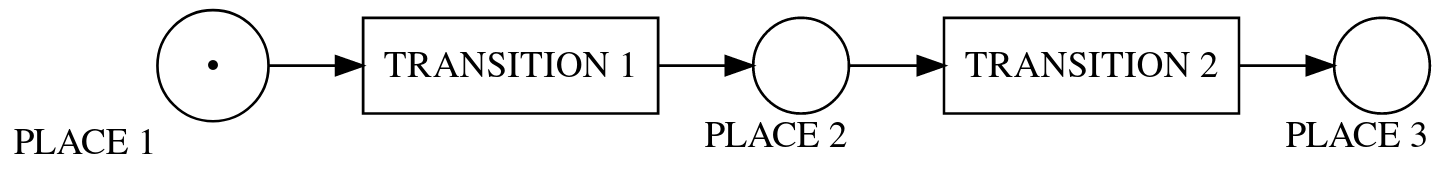
\includegraphics[scale=0.25]{petri-net-example.png}
    \caption{Example of a Petri net. \uppercase{PLACE 1} contains a token.}
    \label{fig:petri-net-example}
\end{figure}

When a transition fires, it consumes tokens from its input places and
produces tokens in its output places, reflecting a change in the state of the system.
The firing of a transition is enabled when there are sufficient tokens in its input places.
In Fig. \ref{fig:petri-net-transition-firing-example}, we can see how successive firings happen.

\begin{figure}[H]
    \centering
    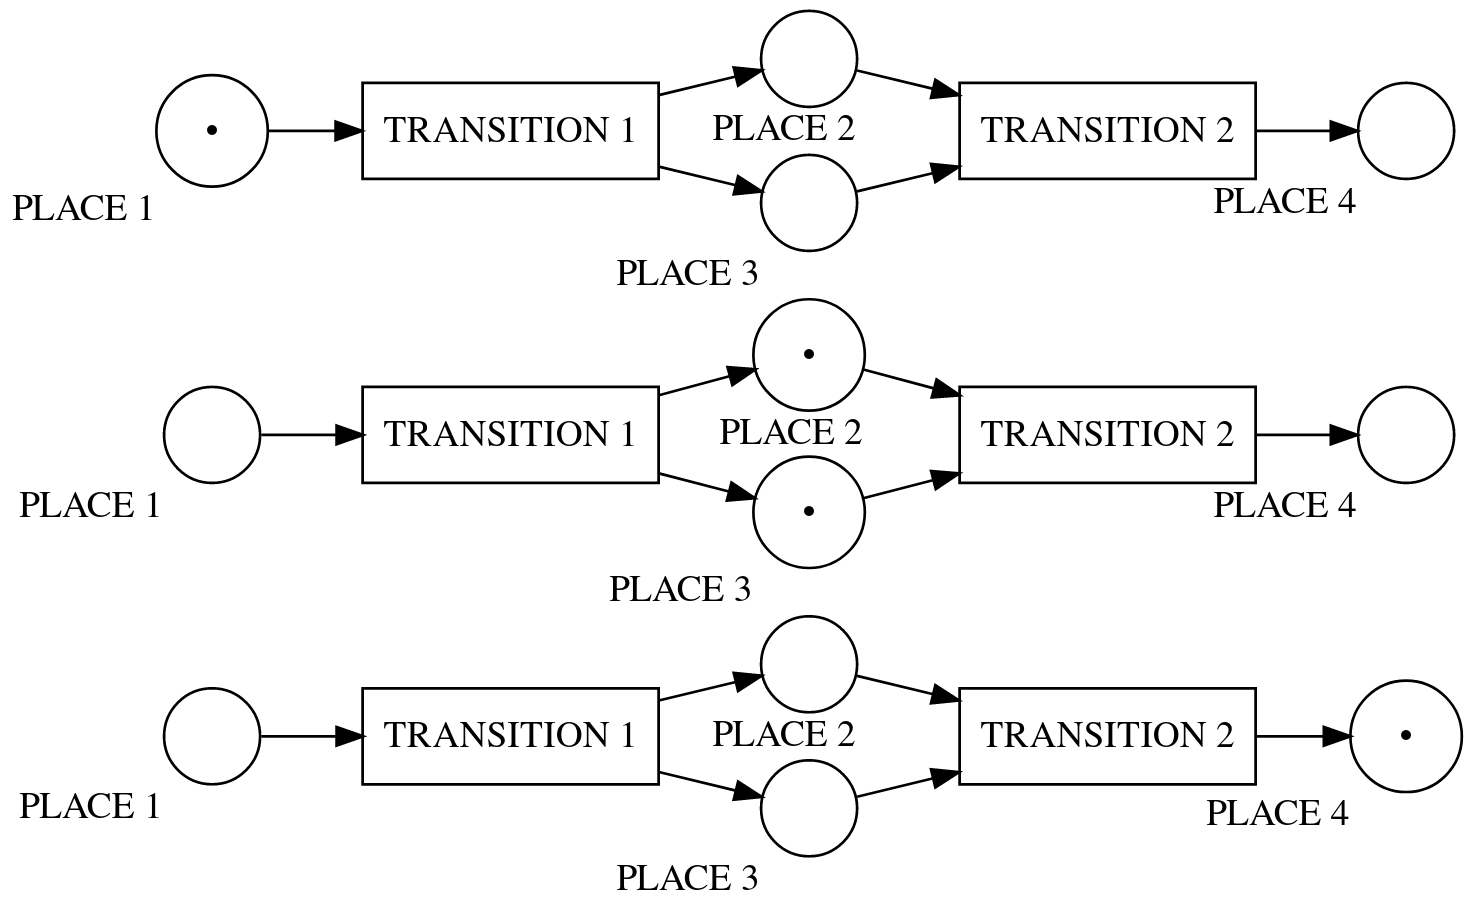
\includegraphics[scale=0.25]{petri-net-transition-firing-example.png}
    \caption{Example of transition firing: Transition 1 fires first, then transition 2 fires.}
    \label{fig:petri-net-transition-firing-example}
\end{figure}

The firing of enabled transitions is not deterministic,
i.e., they fire randomly as long as they are enabled.
A disabled transition is considered \emph{dead}
if there is no reachable state in the system that can lead to the transition being enabled.
If all the transitions in the net are dead, then the net is considered \emph{dead} too.
This state is analogous to the deadlock of a computer program.

Petri nets can be used to model and analyze a wide range of systems,
from simple systems with a few components to complex systems with many interacting components.
They can be used to detect potential problems in a system,
optimize system performance, and design and implement systems more effectively.

They can also be used to model industrial processes \cite{aalst1994putting},
to validate software requirements expressed as use cases \cite{silva2004applying}
or to specify and analyze real-time systems \cite{kavi1996specification}.

In particular, Petri nets can be used to detect deadlocks in source code
by modeling the input program as a Petri net and then analyzing the structure of the resulting net.
It will be shown that this approach is formally sound and
practicably amenable to source code written in the Rust programming language.

\subsection{Formal mathematical model}

A Petri net is a particular kind of bipartite, weighted, directed graph,
equipped with an initial state called the \emph{initial marking}, $M_{0}$.
For this work, the following general definition of a Petri net
taken from \cite{murata1989} will be used.

\begin{definition}{Petri net}{petri-net}
    A Petri net is a 5-tuple, $ PN = (P, T, F, W, M_{0}) $ where:

    \begin{quote}
        $ P = \{ p_1, p_2, \dots, p_m \} $ is a finite set of places,\\
        $ T = \{ t_1, t_2, \dots, t_n \} $ is a finite set of transitions,\\
        $ F \subseteq (P \times T) \cup (T \times P) $ is a set of arcs (flow relation),\\
        $ W: F \leftarrow \{1, 2, 3, ... \} $ is a weight function for the arcs,\\
        $ M_{0}: P \leftarrow \{0, 1, 2, 3, .... \} $ is the initial marking,\\
        $ P \cap T = \varnothing $ and $ P \cup T \neq \varnothing $
    \end{quote}
\end{definition}

In the graphical representation, arcs are labeled with their weight,
which is a non-negative integer $k$.
Usually, the weight is omitted if it is equal to 1.
A $k$-weighted arc can be interpreted as a set of $k$ distinct parallel arcs.

A \emph{marking (state)} associates with each place a non-negative integer $l$.
If a marking assigns to place $p$ a non-negative integer $l$,
we say that $p$ is \emph{marked with $l$ tokens}.
Pictorially, we denote his by placing $l$ black dots (tokens) in place $p$.
The \emph{pth} component of $M$, denoted by $M(p)$, is the number of tokens in place $p$.

An alternative definition of Petri nets uses \emph{bags} instead of a set to define the arcs,
thus allowing multiple elements to be present.
It can be found in the literature, e.g., \cite[Definition 2.3]{peterson1981}.

As an example, consider the Petri net $ PN_{1} = (P, T, F, W, M) $ where:

\begin{quote}
    $ P = \{ p_1, p_2 \} $,\\
    $ T = \{ t_1, t_2 \} $,\\
    $ F = \{ (p_1, t_1), (p_2, t_2), (t_1, p_2), (t_2, p_2) \} $,\\
    $ W(a_i) = 1 \quad \forall a_i \in F $\\
    $ M(p_1) = 0, M(p_2) = 0 $
\end{quote}

This net contains no tokens and all the arc weights are equal to 1.
It is shown in Fig. \ref{fig:petri-net-formal-example}.

\begin{figure}[H]
    \centering
    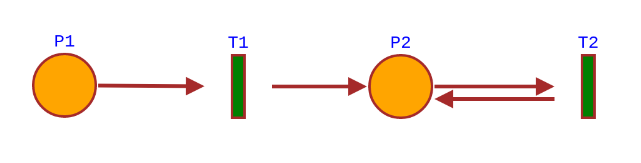
\includegraphics[scale=0.50]{petri-net-formal-example.png}
    \caption{Example of a small Petri net containing a self-loop.}
    \label{fig:petri-net-formal-example}
\end{figure}

Fig. \ref{fig:petri-net-formal-example} contains an interesting structure
that we will encounter later.
This motivates the following definition.

\begin{definition}{Self-loop}{self-loop}
    A place node $p$ and a transition node $t$ define a self-loop
    if $p$ is both an input place and an output place of $t$.
\end{definition}

In most cases, we are interested in Petri nets containing no self-loops,
which are called \emph{pure}.

\begin{definition}{Pure Petri net}{pure-petri-net}
    A Petri net is said to be pure if it has no self-loops.
\end{definition}

Moreover, if every arc weight is equal to one, we call the Petri net \emph{ordinary}.

\begin{definition}{Ordinary Petri net}{ordinary-petri-net}
    A Petri net is said to be ordinary if all of its arc weights are 1's, i.e.
    \begin{equation*}
        W(a) = 1 \quad \forall a \in F
    \end{equation*}
\end{definition}

\subsection{Transition firing}
\label{sec:transition-firing}

The transition firing rule is the core concept in Petri nets.
Despite being deceptively simple, its implications are far-reaching and complex.

\begin{definition}{Transition firing rule}{transition-firing-rule}
    Let $ PN = (P, T, F, W, M_{0}) $ be a Petri net.
    \begin{enumerate}[label=(\roman*)]
        \item A transition $t$ is said to be enabled if each input place $p$ of $t$
              is marked with at least $W(p, t)$ tokens,
              where $W(p,t)$ is the weight of the arc from $p$ to $t$.
        \item An enabled transition may or may not fire,
              depending on whether or not the event takes place.
        \item A firing of an enabled transition $t$ removes
              $W(t,p)$ tokens from each input place $p$ of $t$,
              where $W(t, p)$ is the weight of the arc from $t$ to $p$.
    \end{enumerate}
\end{definition}

Whenever several transitions are enabled for a given marking $M$,
any one of them can be fired.
The choice is nondeterministic.
Two enabled transitions are said to be in \emph{conflict}
if the firing of one of the transitions will disable the other transition.
In this case, the transitions compete for the token placed in a shared input place.

If two transitions $t_1$ and $t_2$ are enabled in some marking but are not in conflict,
they can fire in either order, i.e. $t_1$ then $t_2$ or $t_2$ then $t_1$.
Such transitions represent events that can occur concurrently or in parallel.
In this sense, the Petri net model adopts an \emph{interleaved model of parallelism}, that is,
the behavior of the system is the result of an arbitrary interleaving of the parallel events.

Transitions without input places or output places receive a special name.

\begin{definition}{Source transition}{source-transition}
    A transition without any input place is called a source transition.
\end{definition}

\begin{definition}{Sink transition}{sink-transition}
    A transition without any output place is called a sink transition.
\end{definition}

It is important to note that a source transition is unconditionally enabled
and produces tokens without consuming any, while the firing of a sink transition
consumes tokens without producing any.

\subsection{Modeling examples}

In this subsection, several simple examples are presented to introduce
some basic concepts of Petri nets that are useful in modeling.
This subsection has been adapted from \cite{murata1989}.

For other modeling examples, such as the mutual exclusion problem,
semaphores as proposed by Edsger W. Dijkstra, the producer/consumer problem
and the dining philosophers problem, the reader is referred to
\cite[Chap. 3]{peterson1981} and \cite{reisig2013}.

\subsubsection{Finite-state machines}

\acrfull{FSM} can be represented by a subclass of Petri nets.

As an example of a finite-state machine, consider a coffee vending machine.
It accepts \EUR{1} or \EUR{2} coins and sells two types of coffee,
the first costs \EUR{3} and the second \EUR{4}.
Assume that the machine can hold up to \EUR{4} and does not return any change.
Then, the state diagram of the machine can be represented
by the Petri net shown in Fig. \ref{fig:state-machine-example}.

\begin{figure}[H]
    \centering
    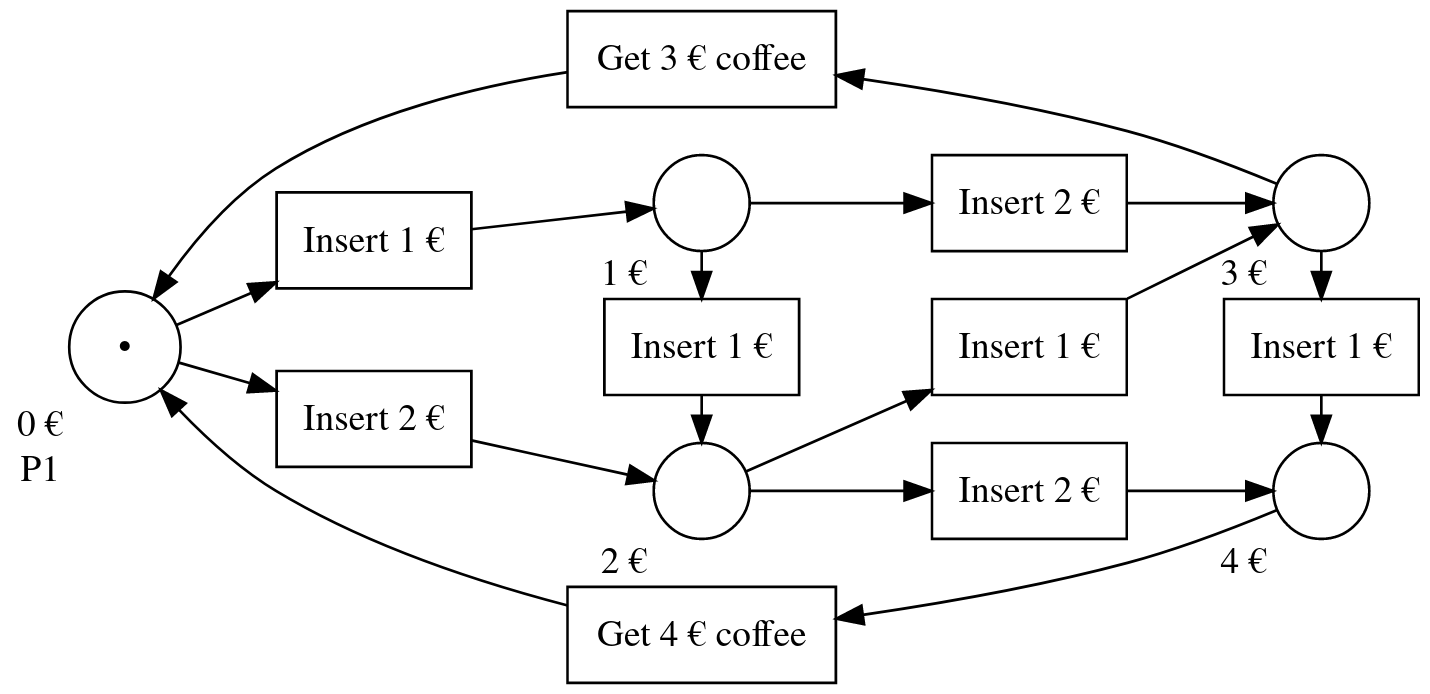
\includegraphics[scale=0.30]{state-machine-example.png}
    \caption{The Petri net for a coffee vending machine.
        It is equivalent to a state diagram.}
    \label{fig:state-machine-example}
\end{figure}

The transitions represent the insertion of a coin of the labeled value,
e.g. ``Insert \EUR{1} coin''.
The places represent a possible state of the machine,
i.e. the amount of money currently stored inside.
The place labeled \uppercase{P1} is marked with a token
and corresponds to the initial state of the system.

We can now present the following definition of this subclass of Petri nets.

\begin{definition}{State machines}{state-machines}
    A Petri net in which each transition has exactly one incoming arc
    and exactly one outgoing arc is known as a state machine.

    Any \acrshort{FSM} (or its state diagram) can be modeled with a state machine.
\end{definition}

The structure of a place $p_1$ having two (or more) output transitions $t_1$ and $t_2$ is called
a \emph{conflict}, \emph{decision}, or \emph{choice}, depending on the application.
This is seen in the initial place \uppercase{P1} of Fig. \ref{fig:state-machine-example},
where the user must select which coin to insert.

\subsubsection{Parallel activities}

Contrary to finite-state machines, Petri nets can also model parallel or concurrent activities.
In Fig. \ref{fig:parallel-activities-example} an example of this is shown,
where the net represents the division of a bigger task
into two subtasks that may be executed in parallel.

\begin{figure}[H]
    \centering
    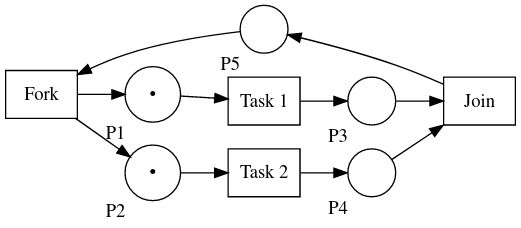
\includegraphics[scale=0.70]{parallel-activities-example.png}
    \caption{The Petri net depicting two parallel activities in a fork-join fashion.}
    \label{fig:parallel-activities-example}
\end{figure}

The transition ``Fork'' will fire before ``Task 1'' and ``Task 2''
and that ``Join'' will only fire after both tasks are complete.
But note that the order in which ``Tast 1'' and ``Tast 2'' execute is non-deterministic.
``Task 1'' could fire before, after, or at the same time that ``Task 2''.
It is precisely this property of the firing rule in Petri nets
that allows the modeling of concurrent systems.

\begin{definition}{Concurrency in Petri nets}{petri-net-concurrency}
    Two transitions are said to be concurrent if they are causally independent, i.e.
    the firing of one transition does not cause and is not triggered by the firing of the other.
\end{definition}

Note that each place in the net in Fig. \ref{fig:parallel-activities-example}
has exactly one incoming arc and one outgoing arc.
This subclass of Petri nets allows the representation of concurrency but not decisions (conflicts).

\begin{definition}{Marked graphs}{marked-graphs}
    A Petri net in which each place has exactly one incoming arc
    and exactly one outgoing arc is known as a marked graph.
\end{definition}

\subsubsection{Communication protocols}

Communications protocols can also be represented in Petri nets.
Fig. \ref{fig:communication-protocols-example} illustrates a simple protocol
in which Process 1 sends messages to Process 2 and
waits for an acknowledgment to be received before continuing.
Both processes communicate through a buffered channel whose maximum capacity is one message.
Therefore, only one message may be traveling between the processes at any given time.
For simplicity, no timeout mechanism was included.

\begin{figure}[H]
    \centering
    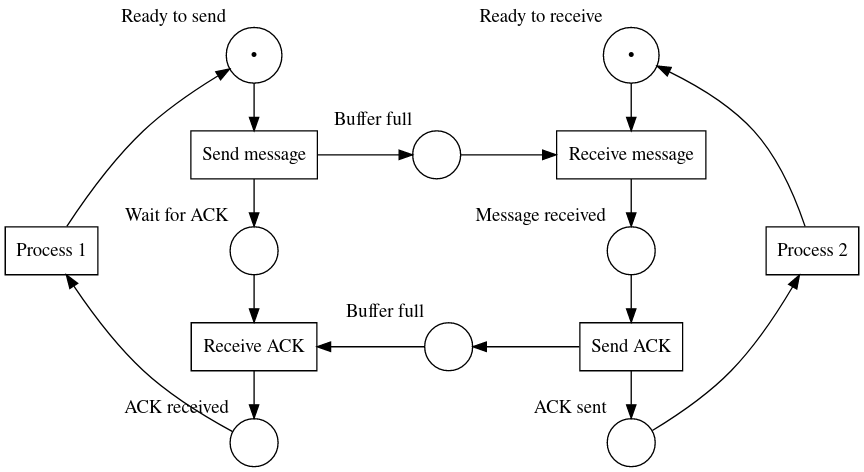
\includegraphics[scale=0.55]{communication-protocols-example.png}
    \caption{A simplified Petri net model of a communication protocol.}
    \label{fig:communication-protocols-example}
\end{figure}

A timeout for the send operation could be incorporated into the model
by adding a transition $t_{timeout}$ with edges from ``Wait for ACK'' to ``Ready to send''.
This maps the decision between receiving the acknowledgment and the timeout.

\subsubsection{Synchronization control}

In a multithreaded system, resources and information are shared among several threads.
This sharing must be controlled or synchronized
to ensure the correct operation of the overall system.
Petri nets have been used to model a variety of synchronization mechanisms,
including the mutual exclusion, readers-writers, and producers-consumers problems \cite{murata1989}.

A Petri net for a readers-writers system with $k$ processes
is shown in Fig. \ref{fig:readers-writers-example}.
Each token represents a process and the choice of T1 or T2
represents whether the process performs a read or a write operation.

It makes use of weighted edges to remove atomically
$k - 1$ tokens from P3 before performing a write (transition T2),
thus ensuring that no readers are present in the right loop of the net.

At most $k$ processes may be reading at the same same,
but when one process is reading, no process is allowed to read, that is P2 will be empty.
It can be easily verified that the mutual exclusion property is satisfied for the system.

\begin{figure}[H]
    \centering
    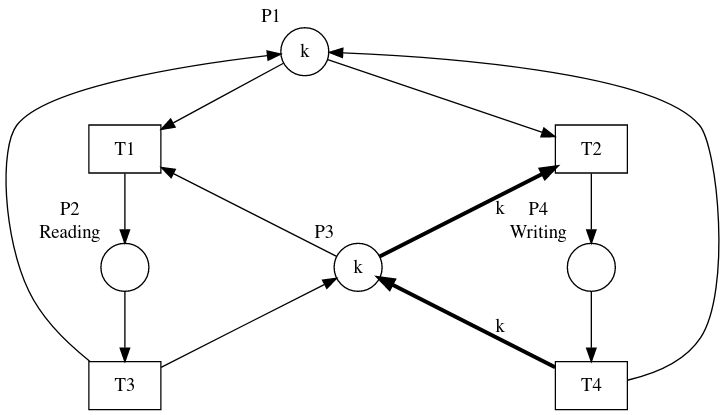
\includegraphics[scale=0.60]{readers-writers-example.png}
    \caption{A Petri net system with k processes that either read or write.}
    \label{fig:readers-writers-example}
\end{figure}

It should be pointed out that this system is not free from starvation,
since there is no guarantee that a write operation will eventually take place.
The system is on the other hand free from deadlocks.

\subsection{Important properties}

In this subsection, we will look at important concepts for the analysis of Petri nets
that will facilitate the understanding of the nets we will be dealing with in the rest of the work.

\subsubsection{Reachability}
\label{sec:reachability}

Reachability is one of the most important questions
when studying the dynamic properties of a system.
The firing of enabled transitions causes changes in the location of the tokens.
In other words, it changes the marking $M$.
A sequence of firings creates a sequence of markings
where each marking may be denoted as a vector of length $n$,
with $n$ being the number of places in the Petri net.

A \emph{firing} or \emph{occurence sequence} is denoted by
$ \sigma = M_0\; t_1\; M_1\; t_2\; M_2\; \cdots\; t_l\; M_l$ or simply
$ \sigma = t_1\; t_2\; \cdots\; t_l\; $, since the markings
resulting from each firing are derived
from the transition firing rule described in Sec. \ref{sec:transition-firing}.

\begin{definition}{Reachability}{reachability}
    We say that a marking $M$ is reachable from $M_0$
    if there exists a firing sequence $\sigma$ such that $M$ is contained in $\sigma$.
\end{definition}

The set of all possible markings reachable from $M_0$ is denoted by $R(N, M_0)$ or more simply
$R(M_0)$ when the net meant is clear.
This set is called the \emph{reachability set}.

A problem of utmost importance in the theory of Petri nets can be presented then,
namely the \emph{reachability problem}:
Finding if $M_n \in R(M_0, N)$ for a given net and initial marking.

In some applications, we are just interested in the markings of a subset of places
and we can ignore the remaining ones.
This leads to a variation of the problem known as the \emph{submarking reachability problem}.

It has been shown that the reachability problem is decidable \cite{mayr1981}.
Nevertheless, it was also shown that it takes exponential space
(formally, it is EXPSPACE-hard) \cite{lipton1976}.
New methods have been proposed to make the algorithms more efficient \cite{kungas2005petri}.
Recently, \cite{czerwinski2020reachability} improved
the lower bound and showed that the problem is not ELEMENTARY.
These results highlight that the reachability problem is still
an active area of research in theoretical computer science.

For this and other key problems, the most important theoretical results
obtained up to 1998 are detailed in \cite{esparza1994decidability}.

\subsubsection{Boundedness and safeness}

During the execution of a Petri net, tokens may accumulate in some places.
Applications need to ensure that the number of tokens in a given place does not
exceed a certain tolerance.
For example, if a place represents a buffer,
we are interested that the buffer will never overflow.

\begin{definition}{Boundedness}{boundedness}
    A place in a Petri net is k-bounded or k-safe
    if the number of tokens in that place can not exceed a finite integer $k$
    for any marking reachable from $M_0$.

    A Petri net is k-bounded or simply bounded if all places are bounded.
\end{definition}

Safeness is a special case of boundedness.
It occurs when the place contains either 1 or 0 tokens during execution.

\begin{definition}{Safeness}{safeness}
    A place in a Petri net is safe if the number of tokens in that place never exceeds one.

    A Petri net is safe if each place in that net is safe.
\end{definition}

The nets in Fig. \ref{fig:state-machine-example}, \ref{fig:parallel-activities-example}
and \ref{fig:communication-protocols-example} are all safe.

The net in Fig. \ref{fig:readers-writers-example}
is k-bounded because all its places are k-bounded.

\subsubsection{Liveness}

The concept of liveness is analogous to
the complete absence of deadlocks in computer programs.

\begin{definition}{Liveness}{liveness}
    A Patri net $(N, M_0)$ is said to be live
    (or equivalently $M_0$ is said to be a live marking for N) if,
    for every marking reachable from $M_0$, it is possible to fire any transition
    of the net by progressing through some firing sequence.
\end{definition}

When a net is live, it can always continue executing,
no matter the transitions that fired before.
Eventually, every transition can be fired again.
If a transition can be fired only once and there is no way to enable it again,
then the net is not live.

This is equivalent to saying that the Petri net is \emph{deadlock-free}.
Let us now define what constitutes a deadlock and show examples of it.

\begin{definition}{Deadlock in Petri nets}{petri-net-deadlock}
    A deadlock in a Patri net is a transition (or a set of transitions) that can not fire
    for any marking reachable from $M_0$.
    The transition (or a set of transitions) can not become enabled again
    after a certain point in the execution.
\end{definition}

A transition is \emph{live} if it is not deadlocked.
If a transition is live, it is always possible to pick a suitable firing
to get from the current marking to a marking that enables the transition.

The nets in Fig. \ref{fig:state-machine-example}, \ref{fig:parallel-activities-example}
and \ref{fig:communication-protocols-example} are all live.
In all these cases, after some firings,
the net returns to the initial state and can restart the cycle.

The net in Fig. \ref{fig:petri-net-example} is not live.
After two firings it finishes executing and nothing more can happen.
The net in Fig. \ref{fig:petri-net-formal-example} is also not live, because
T1 will only execute once and only T2 can be enabled from that point on.

\subsection{Reachability Analysis}

Having introduced the reachability set $R(N, M_0)$ in Sec. \ref{sec:reachability},
we can now present a major analysis technique for Petri nets: the \emph{reachability tree}.

We will run the algorithm for constructing the reachability tree step by step
and then present its advantages and drawbacks.
In general terms, the reachability tree has the following structure:
Nodes represent markings generated from $M_0$, the root of the tree, and its successors.
Each arc represents a transition firing, which transforms one marking into another.

\begin{figure}[!htb]
    \centering
    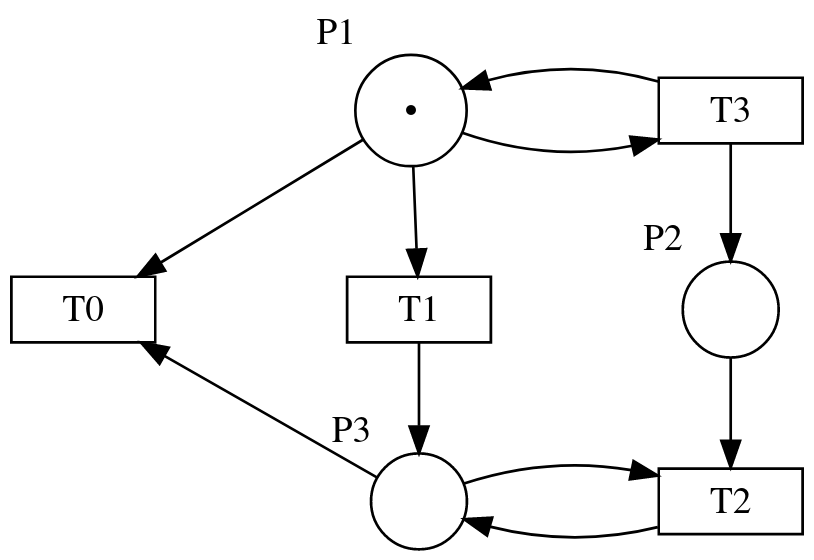
\includegraphics[scale=0.30]{reachability-tree-example.png}
    \caption{A marked Petri net for illustrating the construction of a reachability tree.}
    \label{fig:reachability-tree-example}
\end{figure}

Consider the Petri net shown in Fig. \ref{fig:reachability-tree-example}.
The initial marking is $(1, 0, 0)$.
In this initial marking, two transitions are enabled: T1 and T3.
Given that we would like to obtain the entire reachability set,
we define a new node in the reachability tree for each reachable marking,
which results from firing each transition.
An arc, labeled by the transition fired, leads from the initial marking
(the root of the tree) to each of the new markings.
After this first step (Fig. \ref{fig:reachability-tree-step-1}),
the tree contains all markings that are immediately reachable from the initial marking.

\begin{figure}[!htb]
    \centering
    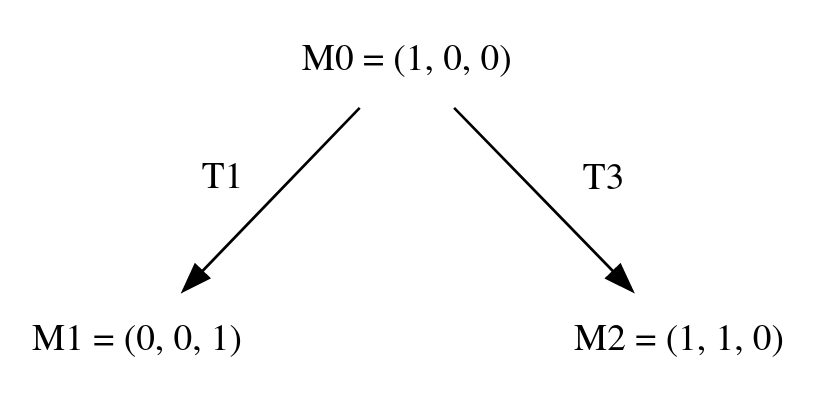
\includegraphics[scale=0.30]{reachability-tree-step-1.png}
    \caption{The first step building the reachability tree
        for the Petri net in Fig. \ref{fig:reachability-tree-example}.}
    \label{fig:reachability-tree-step-1}
\end{figure}

Now we must consider all markings reachable from the leaves of the tree.

From marking $(0,0,1)$ we can not fire any transition.
This is known as a \emph{dead marking}.
In other words, it is a ``dead-end'' node.
This class of end-states is particularly relevant for deadlock analysis.

From the marking on the right of the tree, denoted $(1, 1, 0)$, we can fire T1 or T3.
If we fire T1, we obtain $(0, 1, 1)$ and if T3 fires, the resulting marking is $(1, 2, 0)$.
This produces the tree of Fig. \ref{fig:reachability-tree-step-2}.

\begin{figure}[!htb]
    \centering
    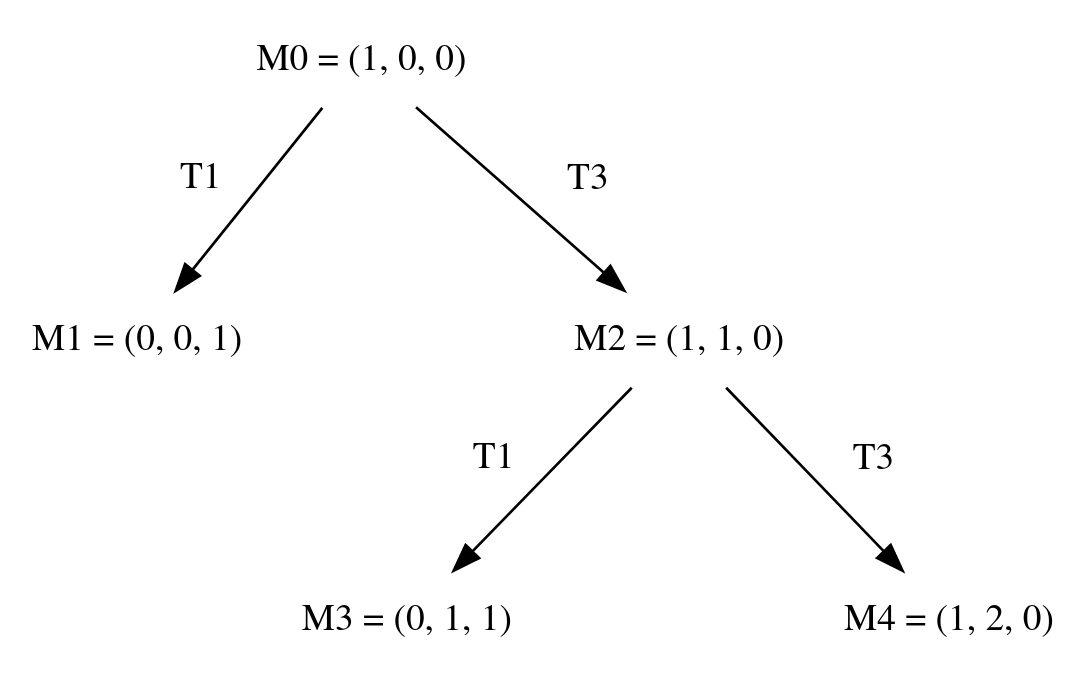
\includegraphics[scale=0.30]{reachability-tree-step-2.png}
    \caption{The second step building the reachability tree
        for the Petri net in Fig. \ref{fig:reachability-tree-example}.}
    \label{fig:reachability-tree-step-2}
\end{figure}

Note that starting with marking $(0, 1, 1)$, only the transition T2 is enabled,
which will lead to a marking $(0, 0, 1)$ that was already seen before.
If instead we take $(1, 2, 0)$ we have again the same possibilities as starting from $(1, 1, 0)$.
It is easy to see that the tree will continue to grow down that path.
The tree is therefore infinite and this is because
the net in Fig. \ref{fig:reachability-tree-example} is not bounded.
See Fig. \ref{fig:reachability-tree-final-step} for the abbreviated final result.

\begin{figure}[!htb]
    \centering
    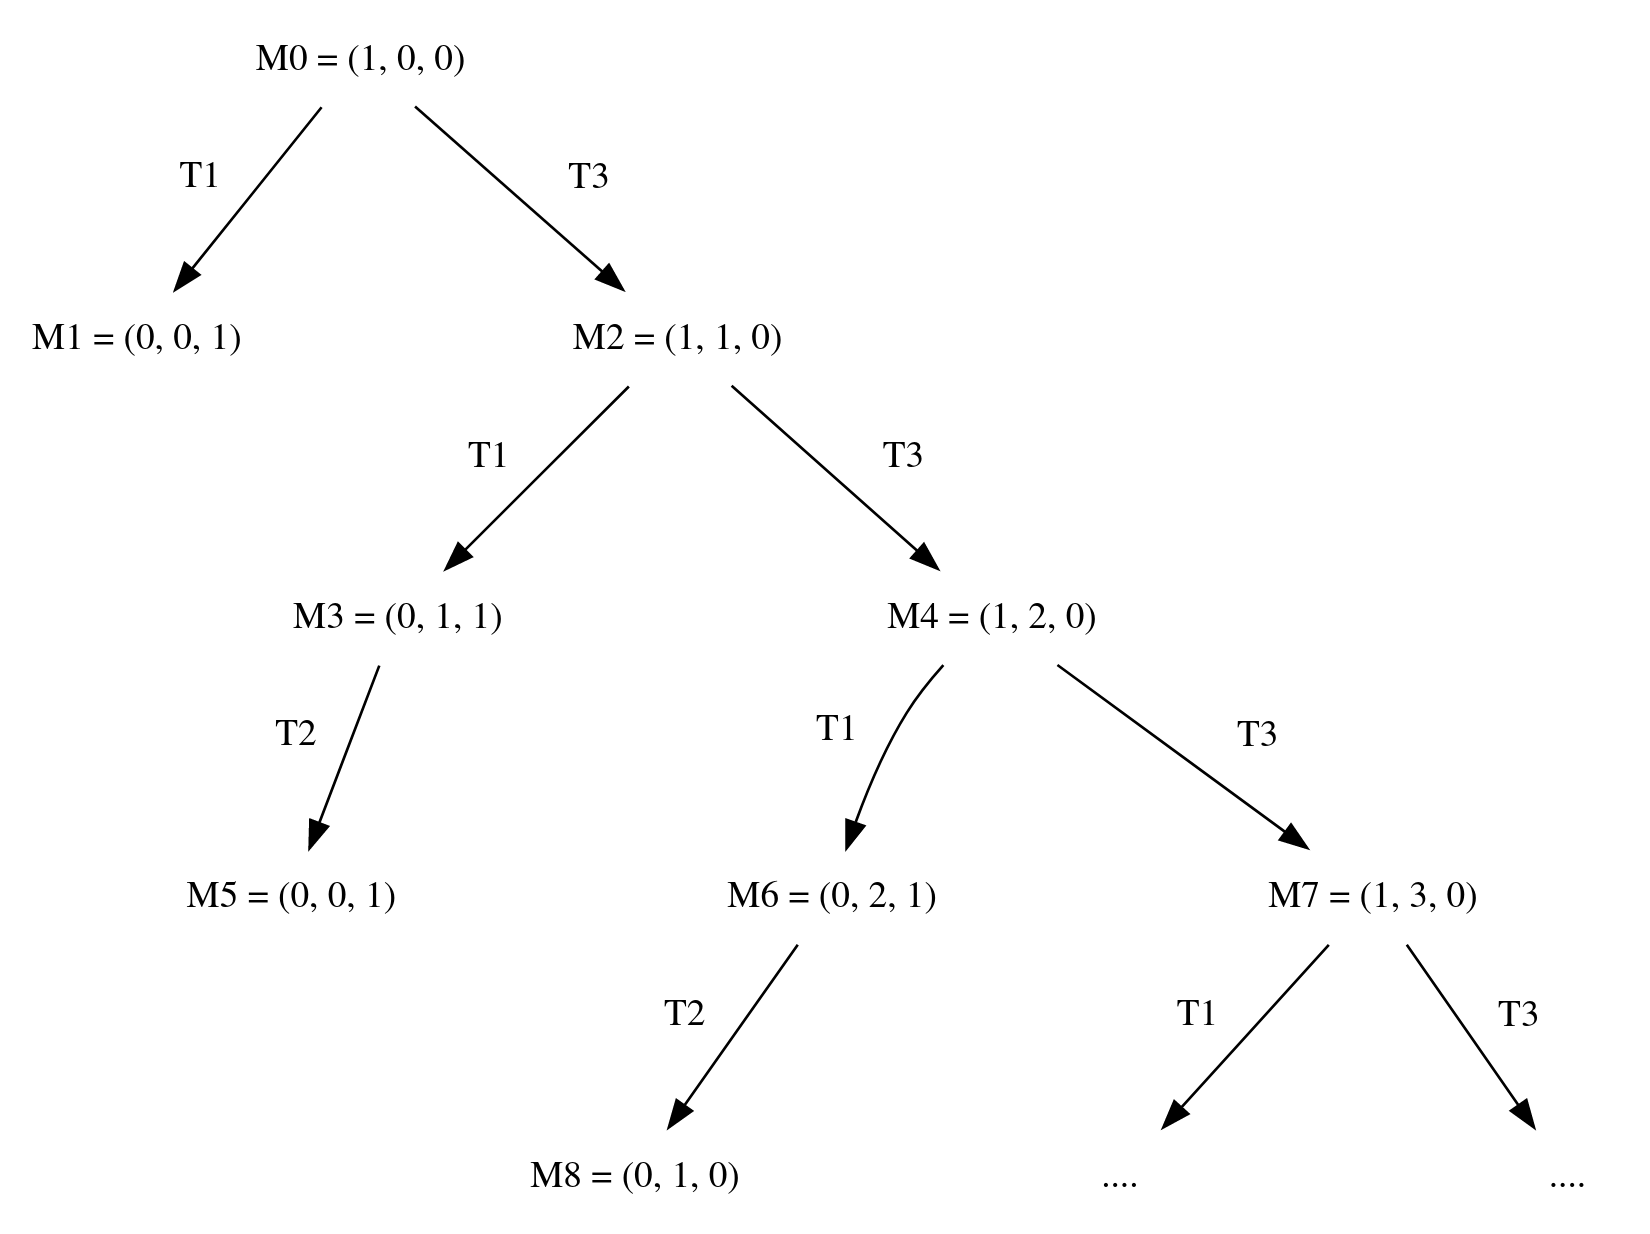
\includegraphics[scale=0.27]{reachability-tree-final-step.png}
    \caption{The infinite reachability tree for the Petri net in Fig.
        \ref{fig:reachability-tree-example}.}
    \label{fig:reachability-tree-final-step}
\end{figure}

The previously presented method enumerates the elements in the reachability set.
Every marking in the reachability set will be produced
and so for any Petri net with an infinite reachability set
(i.e. an infinite number of possible states),
the corresponding tree would also be infinite.
Nonetheless, this opposite is not true.
A Petri net with a finite reachability set can have an infinite tree
(see Fig. \ref{fig:reachability-tree-bounded-net-counterexample}).
This net is even \emph{safe}.
In conclusion, dealing with a bounded or safe net is not
a guarantee that the total number of reachable states will be finite.

\begin{figure}[!htb]
    \centering
    \begin{subfigure}
        \centering
        % https://stackoverflow.com/questions/2328403/vertical-alignment-of-subfigures-latex
        \raisebox{3.5cm}{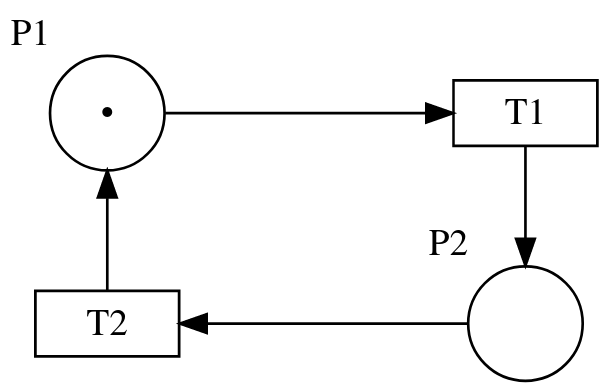
\includegraphics[scale=0.30]{petri-net-loop.png}}
    \end{subfigure}
    % Horizontal space between the figures. \hfill is too much.
    \hspace{1.5cm}
    \begin{subfigure}
        \centering
        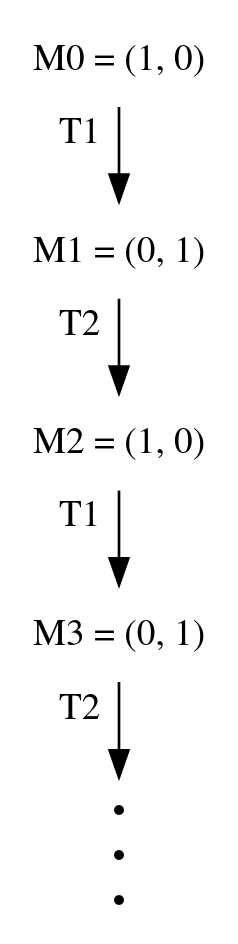
\includegraphics[scale=0.30]{reachability-tree-bounded-net-counterexample.png}
    \end{subfigure}
    \caption{A simple Petri net with an infinite reachability tree.}
    \label{fig:reachability-tree-bounded-net-counterexample}
\end{figure}

For the reachability tree to be a useful analysis tool,
it is necessary to devise a method to limit it to a finite size.
This implies in general a certain loss of information since the method will have to map
an infinite number of reachable markings onto a single element.
The reduction to a finite representation may be accomplished by the following means.

Notice on one hand that we may encounter duplicate nodes
in our tree and we always naively treat them as new.
This is illustrated most clearly in Fig. \ref{fig:reachability-tree-bounded-net-counterexample}.
It is thus possible to stop the exploration of the successors of a duplicated node.

Notice on the other hand that some markings are strictly different from previously seen markings
but they enable the same set of transitions.
We say in this case that the marking with additional tokens \emph{covers} the one
that has the minimum number of tokens needed to enable the set of transitions in question.
Firing some transitions may allow us to accumulate an arbitrary number of tokens in one place.
For example, firing T3 in the Petri net seen in
Fig. \ref{fig:reachability-tree-example} exhibits exactly this behavior.
Therefore, it would suffice to mark the accumulating place
with a special label $\omega$, which stands for infinity
since we could get as many tokens as we wish in that place.

For instance, the result of converting the tree of Fig. \ref{fig:reachability-tree-final-step}
to a finite tree is shown in Fig. \ref{fig:reachability-tree-final-step-finite}.

\begin{figure}[!htb]
    \centering
    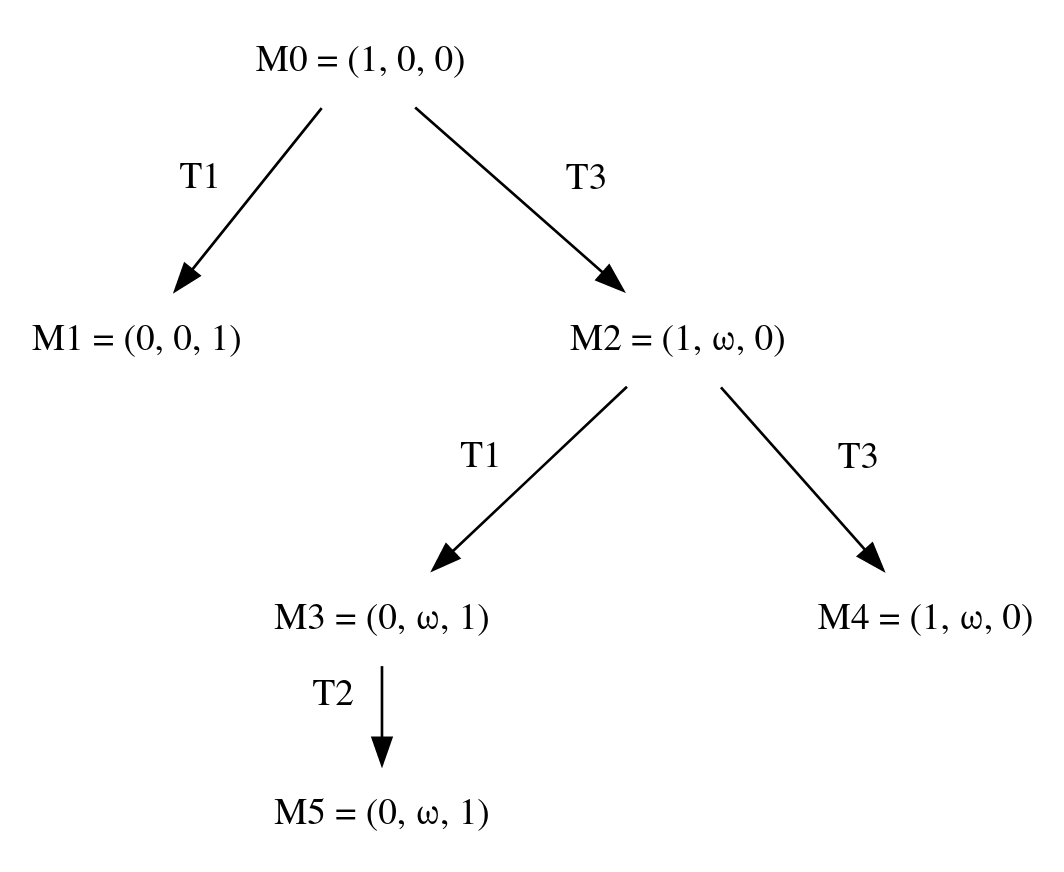
\includegraphics[scale=0.30]{reachability-tree-final-step-finite.png}
    \caption{The finite reachability tree for the Petri net in Fig.
        \ref{fig:reachability-tree-example}.}
    \label{fig:reachability-tree-final-step-finite}
\end{figure}

For more details about

\begin{enumerate}
    \item the technique for representing infinite reachability trees using $\omega$,
    \item a definition of the algorithm and precise steps for constructing the reachability tree,
    \item mathematical proof that the reachability tree generated by it is finite,
    \item and the distinction between the reachability tree and the \emph{reachability graph}
\end{enumerate}

the reader is referred to \cite{murata1989} and \cite{peterson1981}.
These concepts are beyond the scope of this work
and are not required in the following chapters.

\end{document}
\section{The Rust programming language}

One of the most promising modern programming languages
for concurrent and memory-safe programming is Rust\footnote{\url{https://www.rust-lang.org/}}.
Rust is a multi-paradigm, general-purpose programming language that aims to provide developers
with a safe, concurrent, and efficient way to write low-level code.
It started as a project at Mozilla Research in 2009.
The first stable release, Rust 1.0, was announced on May 15, 2015.
For a brief history of Rust up to 2023, see \cite{thompson2023mit}.

Rust's memory model based on the concept of \emph{ownership} and its expressive type system prevent
a wide variety of error classes related to memory management and concurrent programming at compile-time:

\begin{itemize}
      \item Double free \cite[Chap. 4.1]{rust-book}
      \item Use after free \cite[Chap. 4.1]{rust-book}
      \item Dangling pointers \cite[Chap. 4.2]{rust-book}
      \item Data races \cite[Chap. 4.2]{rust-book}
            (with some important caveats explained in \cite[Chap. 8.1]{rustonomicon})
      \item Passing non-thread-safe variables \cite[Chap. 16.4]{rust-book}
\end{itemize}

The official compiler \emph{rustc}\footnote{\url{https://github.com/rust-lang/rust}}
takes care of controlling how the memory is used and allocating and deallocating objects.
If a violation of its strict rules is found, the program will simply not compile.

In this section, we will justify the choice of Rust
to study the detection of deadlocks and lost signals.
We will show how these problems can be studied separately,
knowing that other errors are already caught at compile time.
In other words, we will argue that
the stability and safety of the language provide a firm foundation
on which to build a tool that detects additional errors during compilation.

\subsection{Main characteristics}

Some of Rust's main features are:

\begin{itemize}
      \item Type system: Rust has a powerful type system
            that provides compile-time safety checks and prevents many common programming errors.
            It includes features such as type inference, generics, enums, and pattern matching.
            Every variable has a type but it is commonly inferred by the compiler.
      \item Performance: Rust's performance is comparable to C and C++,
            and it is often faster than many other popular programming languages
            such as Java, Go, Python, or Javascript.
            Rust's performance is achieved through a combination of features
            such as zero-cost abstractions, minimal runtime, and efficient memory management.
      \item Concurrency: Rust has built-in support for concurrency.
            It supports several concurrency paradigms such as shared state,
            message passing and asynchronous programming.
            It does not force the developer to implement concurrency in a specific manner.
      \item Ownership and borrowing: Rust uses a unique ownership model to manage memory,
            allowing for efficient memory allocation and deallocation
            without the risk of memory leaks or data races.
            Furthermore, it does not rely on a garbage collector, thus saving resources.
            The \emph{borrow checker} ensures that
            there is only one owner of a resource at any given time.
      \item Community-driven: Rust has a vibrant and growing community of developers
            who contribute to the language's development and ecosystem.
            Anyone can contribute to the language's development and suggest improvements.
            The documentation is also open-source and significant decisions are documented
            in the form of \acrfull{RFCs}\footnote{\url{https://rust-lang.github.io/rfcs/}}.
\end{itemize}

The release cycle of the official Rust compiler, \textit{rustc}, is remarkably fast.
A new stable version of the compiler is released every 6 weeks \cite[Appendix G]{rust-book}.
This is made possible by a complex automated testing system that compiles even all packages
available on \texttt{crates.io}\footnote{\url{https://crates.io/}}
using a program called \textit{crater}\footnote{\url{https://github.com/rust-lang/crater}}
to verify that compiling and running the tests with the new version of the compiler
does not break existing packages \cite{albini2019}.

\subsubsection{The borrow checker}

Rust's borrow checker is an essential component of its ownership model,
which is designed to ensure memory safety and prevent data races in concurrent code.
The borrow checker analyzes Rust code at compile-time
and enforces a set of rules to ensure that a program's memory is accessed safely and efficiently.

The core idea behind the borrow checker is that
each piece of memory in a Rust program has an owner.
The owner may change during execution but
there can only be one owner at any given time.
Memory values can also be \emph{borrowed}, that is,
used without swapping the owner,
similar to accessing the value through a pointer
or a reference in other programming languages.
When a value is borrowed, the borrower receives a reference to the value,
but the original owner retains ownership.
The borrow checker enforces rules to ensure that
a borrowed value is not modified while it is borrowed
and that the borrower releases the reference before the owner goes out of scope.

For clarity, we will now present some of the key rules enforced by the borrow checker:

\begin{itemize}
      \item No two mutable references to the same memory location can exist simultaneously.
            This prevents data races, where two threads
            try to modify the same memory location at the same time.
      \item Mutable references cannot exist at the same time
            as immutable references to the same memory location.
            This ensures that mutable and immutable references
            cannot be used simultaneously, preventing inconsistent reads and writes.
      \item References cannot outlive the value they reference.
            This ensures that references do not point to invalid memory locations,
            preventing null pointer dereferences and other memory errors.
      \item References cannot be used after their owner has been moved or destroyed.
            This ensures that references do not point to memory that has been deallocated,
            preventing use-after-free errors.
\end{itemize}

It can take some effort to write Rust code that satisfies these rules.
The borrow checker is usually singled out as
one aspect of the language that is confusing for newcomers.
However, this discipline pays off in terms of
increased memory safety and performance.
By ensuring that Rust programs follow these rules,
the borrow checker eliminates many common programming errors
that can lead to memory leaks, data races, and other bugs,
while also teaching good coding practices and patterns.

\subsubsection{Error handling enforced by the compiler}

Error handling is an essential aspect of programming and
is typically addressed in the design of programming languages.
The myriad of approaches can be summarized in two separate groups.

One group formed by languages such as C++, Java, or Python employs exceptions,
utilizing \texttt{try} and \texttt{catch} blocks to handle exceptional conditions.
When exceptions are thrown and not caught, the program terminates abruptly.

The other group is formed by languages like C or Go, among others,
where the convention is to communicate an error either through the return value of functions
or through a function parameter specifically dedicated to this purpose.
The disadvantage is that the compiler does not enforce error-checking on the programmer,
which may lead to error cases not being taken into account when adding new functionality.

Rust takes a different approach by promoting the notion that functions should ideally not fail
and that the function signature should reflect if the function may return an error.
Instead of exceptions or integer error codes,
Rust functions that may encounter errors return a
\Rustinline{std::result::Result}\footnote{\url{https://doc.rust-lang.org/std/result/}} type,
which can hold either the result of the computation
or a custom error type accompanied by a description of the error.
\emph{rustc} requires the programmer to write code for both cases
and the language provides mechanisms to facilitate error handling \cite[Chap. 9.2]{rust-book}.

In Rust, the focus lies on consistently managing the error case.
Errors can be propagated to higher-level function calls
until a consistent program state can be restored.
However, there may be situations where recovery from an error state is not feasible.
In such cases, the program can be instructed to panic,
resulting in an abrupt and ungraceful shutdown,
similar to an uncaught exception in other programming languages.
During a panic, program execution is aborted, and the stack is unwound \cite[Chap. 9.1]{rust-book}.
An error message containing details of the panic,
e.g., the error message itself and its location, is generated.
While panics can be caught by parent threads and
in specific cases when the programmer so desires\footnote{\url{https://doc.rust-lang.org/std/panic/fn.catch\_unwind.html}},
they typically lead to the termination of the current program.
This structured panic mechanism ensures that
the compiler is aware of potential unrecoverable errors,
enabling the generation of appropriate code to handle such cases.

Rust also provides a type \Rustinline{std::option::Option}\footnote{\url{https://doc.rust-lang.org/std/option/}}
that represents either the presence of a value or the absence of it.
The compiler again enforces discipline on the programmer to always handle the \Rustinline{None} case.
Thus, Rust eliminates almost completely the need for a NULL pointer
as found in other languages like C, C++, Java, Python, or Go.

\subsection{Adoption}

In this subsection, we will briefly describe the trend
in the adoption of the Rust programming language.
This highlights the relevance of this work
as a contribution to a growing community of programmers
who emphasize the importance of safe and performant systems programming
for the next years in the software industry.

In the last few years, several major projects in the Open Source community and
at private companies have decided to incorporate Rust to reduce the number of bugs
related to memory management without sacrificing performance.
Among them, we can name a few representative examples:

\begin{itemize}
      \item The Android Open Source Project encourages
            the use of Rust for the SO components
            below the \acrfull{ART} \cite{stoep2021}.
      \item The Linux kernel, which introduces in version 6.1
            (released in December 2022) official tooling
            support for programming components in Rust
            \cite{corbet2022,desimone2022}.
      \item At Mozilla, the Oxidation project was created in 2015
            to increase the usage of Rust in Firefox and related projects.
            As of March 2023, the lines of code in Rust represent more than
            10\% of the total in Firefox Nightly \cite{mozilla-oxidation}.
      \item At Meta, the use of Rust as a development language server-side
            is approved and encouraged since July 2022 \cite{garcia2022}.
      \item At Cloudflare, a new HTTP proxy in Rust was built from scratch
            to overcome the architectural limitations of NGINX,
            reducing CPU usage by 70\% and memory usage by 67\% \cite{wu2022}.
      \item At Discord, reimplementing a crucial service written in Go
            in Rust provided great benefits in performance
            and solved a performance penalty due to the garbage collection in Go \cite{howarth2020}.
      \item At npm Inc., the company behind the npm registry, Rust allowed scaling CPU-bound services
            to more than 1.3 billion downloads per day \cite{rust-npm-case-study}.
\end{itemize}

In other cases, Rust has proved to be a great choice in existing C/C++ projects to rewrite modules
that process untrusted user input, for instance, parsers,
and reduce the number of security vulnerabilities due to memory issues \cite{chifflier2017writing}.

Moreover, the interest of the developer community in Rust is undeniable,
as it has been rated for 7 years in a row as the programming language most ``loved'' by programmers
in the Stack Overflow Developer Survey \cite{so-survey2022}.

\subsection{Importance of memory safety}

In this subsection, compelling evidence supporting
the use of a memory-safe programming language is presented.
The goal is to highlight the importance of advancing research in the compile-time detection of errors
to prevent bugs that are subsequently difficult to correct in production systems.

Several empirical investigations have concluded that around 70\% of the vulnerabilities
found in large C/C++ projects occur due to memory handling errors.
This high figure can be observed in projects such as:

\begin{itemize}
      \item Android Open Source Project \cite{memory-bugs-android},
      \item the Bluetooth and media components of Android \cite{memory-bugs-android-media-bluetooth},
      \item the Chromium Projects behind the Chrome web browser \cite{memory-bugs-chrome},
      \item the CSS component of Firefox \cite{memory-bugs-firefox},
      \item iOS and macOS \cite{memory-bugs-ios-macos},
      \item Microsoft products \cite{miller-security-microsoft2019, memory-bugs-microsoft},
      \item Ubuntu \cite{memory-bugs-ubuntu}
\end{itemize}

Numerous tools have set the goal to address these vulnerabilities
caused by improper memory allocation in already established codebases.
However, their use leads to a noticeable loss of performance and
not all vulnerabilities can be prevented \cite{szekeres2013sok}.
An example of a representative tool in this area, more precisely
a dynamic data racer detector for multithreaded programs in C,
can be found in \cite{savage1997eraser},
whose algorithm was later improved in \cite{jannesari2009helgrind+} and
integrated into the Helgrind tool, part of the well-known
Valgrind instrumentation framework\footnote{\url{https://valgrind.org/}}.

In \cite{jaeger2014mind}, the authors provide
a detailed survey of programming language features that
compromise the security of the resulting programs.
They discuss the intrinsic security characteristics of programming languages
and list recommendations for the education of developers or evaluators for secure software.
Type safety is mentioned as one of the key elements
for eliminating complete classes of bugs from the start.
Another noteworthy consideration is using a language where the specifications are
as complete, explicit, and formally defined as possible.
The concept of \acrfull{UB} should be included with caution and only sparingly.
Examples from the C/C++ specification illustrate the confusion
that follows from not following these principles.
The authors conclude that memory safety achieved
through garbage collection poses a threat to security
and that other mechanisms should be considered instead.

We must note that Rust itself, like any other piece of software,
is not exempt from security vulnerabilities.
Serious bugs have been discovered in the standard library in the past \cite{davidoff2018}.
Besides, code generation in Rust also includes mitigations
to exploits of various kinds \cite[Chap. 11]{rustc-book}.
However, this is far from the well-known issues in C and C++.
\section{Correctness of concurrent programs}

In the area of concurrent computing, one of the main challenges is
to prove the correctness of a concurrent program.
Unlike a sequential program where for each input the same output
is always obtained, in a concurrent program the output may depend
on how instructions from different processes or
threads were interleaved during execution.

The correctness of a concurrent program is then defined
in terms of the properties of the computation performed
and not only in terms of the obtained result.
In the literature \cite{ben-ari2006,coulouris2012,tanenbaum2017},
two types of correctness properties are defined:

\begin{itemize}
    \item \textbf{Safety properties}: The property must \emph{always} be true.
    \item \textbf{Liveness properties}: The property must \emph{eventually} become true.
\end{itemize}

Two desirable safety properties in a concurrent program are:

\begin{itemize}
    \item \textbf{Mutual exclusion}: Two processes must not access shared resources at the same time.
    \item \textbf{Absence of deadlock}: A running system must be able to continue performing its task,
          that is, progressing and producing useful work.
\end{itemize}

Synchronization primitives such as mutexes,
semaphores (as proposed by \cite{Dijkstra2002}),
monitors (as proposed by \cite{hansen1972structured,hansen1973operating}),
and condition variables (as proposed by \cite{hoare1974monitors}) are usually used
to implement coordinated access of threads or processes to shared resources.
However, the correct use of these primitives is difficult to achieve in practice
and can introduce errors that are difficult to detect and correct.
Currently, most general-purpose languages, whether compiled or interpreted,
do not allow these errors to be detected in all cases.

Given the increasing importance of concurrent programming due to the proliferation
of multithreaded and multithreaded hardware systems,
minimizing the occurrence of errors associated with thread or process synchronization
holds significant importance for the industry.
Deadlock-free operation is an unavoidable requirement for many projects, such as
operating systems \cite{ArpaciDusseau2018}, autonomous vehicles \cite{Perronnet2019}
and aircraft \cite{carreno2005safety,monzon2009deadlock}.

In the next section, we will have a closer look at the conditions that cause a deadlock
and the strategies used to cope with them.
\section{Deadlocks}

Deadlocks are a common problem that can occur in concurrent systems,
which are systems where multiple threads or processes are
running simultaneously and potentially sharing resources.
They have been studied at least since \cite{dijkstra1964},
who coined the term ``deadly embrace'' in Dutch, which did not catch on.

A deadlock occurs when two or more threads or processes
are blocked and unable to continue executing
because each is waiting for the other to release a resource that it needs.
This results in a situation where none of the threads or processes
can make progress and the system becomes effectively stuck.
An alternative equivalent definition of deadlocks
in terms of program states can be found in \cite{holt1972some}.

Deadlocks can be a serious problem in concurrent systems,
as they can cause the system to become unresponsive or even crash.
Therefore, it is important to be able to detect and prevent deadlocks.
They can occur in any concurrent system where multiple threads or processes
are competing for shared resources.
Examples of shared resources that can lead to deadlocks include system memory,
input/output devices, locks, and other types of synchronization primitives.

Deadlocks can be difficult to detect and prevent
because they depend on the precise timing of events in the system.
Even in cases where deadlocks can be detected, resolving them can be difficult,
as it may require releasing resources that have already been acquired or
rolling back completed transactions.
To avoid deadlocks, it is important to carefully
manage shared resources in a concurrent system.
This can involve using techniques such as resource allocation algorithms,
deadlock detection algorithms, and other types of synchronization primitives.
By carefully managing shared resources,
it is possible to prevent deadlocks from occurring and
ensure the smooth operation of concurrent systems.

To understand the concept in more detail,
consider a simple example where two processes, A and B,
are competing for two resources, X and Y.
Initially, process A has acquired resource X and is waiting to acquire resource Y,
while process B has acquired resource Y and is waiting to acquire resource X.
In this situation, neither process can continue executing
because it is waiting for the other process to release a resource that it needs.
This results in a deadlock, as neither process can make progress.
Fig. \ref{fig:state-graph-example} illustrates this situation.
The cycle therein indicates a deadlock, as will be explained in the next section.

\begin{figure}[!htb]
    \centering
    \includesvg[width=0.3\linewidth]{state-graph-example.svg}
    \caption{Example of a state graph with a cycle indicating a deadlock.}
    \label{fig:state-graph-example}
\end{figure}
\subsection{Necessary conditions}
\label{sec:coffman-conditions}

According to the classic paper on the topic \cite{coffman1971deadlocks},
the following conditions need to hold for a deadlock to arise.
They are sometimes called ``Coffman conditions''.

\begin{enumerate}
    \item \textbf{Mutual Exclusion}: At least one resource in the system must
          be held in a non-sharable mode, meaning that only one thread or process can use it at a time
          (e.g. a variable behind a mutex).
    \item \textbf{Hold and Wait}: At least one thread or process in the system must
          be holding a resource and waiting to acquire additional resources
          that are currently being held by other threads or processes.
    \item \textbf{No Preemption}: Resources cannot be preempted, which means that a thread or process
          holding a resource cannot be forced to release it until it has completed its task.
    \item \textbf{Circular Wait}: There must be a circular chain of two or more threads or processes,
          where each thread or process is waiting for a resource held by the next one in the chain.
          This is usually visualized in a graph representing the order in which the resources are acquired.
\end{enumerate}

Usually, the first three conditions are characteristics of the system under study, i.e.
the protocols used for acquiring and releasing resources,
while the fourth may or may not occur depending
on the interleaving of instructions during the execution.

It is worth noting that the Coffman conditions are in general necessary
but not sufficient for a deadlock to occur.
The conditions are indeed sufficient in the case of single-instance resource systems.
But they only indicate the possibility of deadlock in systems
where there are multiple indistinguishable instances of the same resource.

In the general case, if any one of the conditions is not met, a deadlock cannot occur,
but the presence of all four conditions does not necessarily guarantee a deadlock.
Nonetheless, the Coffman conditions are an important tool for understanding and
analyzing the causes of deadlocks in concurrent systems
and they can help guide the development of strategies for preventing and resolving deadlocks.

\subsection{Strategies}
\label{sec:deadlock-strategies}

Several strategies for handling deadlocks exist,
each of which has its strengths and weaknesses.
In practice, the most effective strategy will depend on the specific requirements
and constraints of the system being developed.
Designers and developers must carefully consider the trade-offs between different strategies
and choose the approach that is best suited to their needs.
Interested readers are referred to \cite{coffman1971deadlocks,singhal1989deadlock}.

\subsubsection{Prevention}

One way to deal with deadlocks is to prevent them from occurring in the first place.
The idea is for deadlocks to be excluded a priori.
With this objective in mind, we must ensure that at every point in time
at least one of the necessary conditions developed in Sec. \ref{sec:coffman-conditions}
is not satisfied.
This restricts the possible protocols in which requests for resources may be made.
We will now look at each condition separately
and elaborate on the most common approaches.

If the first condition must be false,
then the program should allow shared access to all resources.
Lock-free synchronization algorithms may be used for this purpose
since they do not implement mutual exclusion.
This is difficult to achieve in practice for all resource types,
since for example a file may not be shared by more than one thread or process
during an update of the file contents.

Looking at the second condition, a feasible approach would be to impose that
each thread or process acquires all the required resources at once and that
the thread or process cannot proceed until access to all of them has been granted.
This all-or-nothing policy causes a significant performance penalty,
given that resources may be allocated to a specific thread or process
but may remain unused for long periods.
In simpler terms, it decreases concurrency.

If the no preemption condition is denied, then resources may be recovered
in certain circumstances, e.g. using resource allocation algorithms that
ensure that resources are never held indefinitely.
After a timeout or when a condition is satisfied,
the thread or process releases the resource
or a supervisor process recovers the resource forcibly.
Usually, this works well when the state of the resource can be easily saved
and restored later.
One example of this is the allocation of CPU cores in a modern \acrfull{OS}.
The scheduler allocates one processor core to one task and
may switch to a different task or
may move the task to a new processor core at any moment just
by saving the contents of the registers \cite[Chap. 6]{ArpaciDusseau2018}.
However, if preserving the resource state is not possible,
preemption may entail a loss of the progress done so far,
which is not acceptable in many scenarios.

Lastly, if the state graph of the resources never forms a cycle,
then the fourth necessary condition is false and deadlocks are prevented.
To achieve this one could introduce a linear ordering of resource types.
In other words, if a process or thread has been allocated resources of type $r_i$,
it may subsequently require only those resources
of types that follow $r_i$ in the ordering.
This involves using special synchronization primitives
that allow resources to be shared in a controlled manner and
enforcing strict rules for resource acquisition and release.
Under these conditions, the state graph will be strictly speaking
a forest (an acyclical graph), thus no deadlocks are possible.

In practical applications, a combination of the previous strategies may prove useful
when none of them is entirely applicable.
\subsubsection{Avoidance}

Avoidance is another strategy for dealing with deadlocks,
which involves dynamically detecting and
avoiding potential deadlocks \emph{before} they occur.
For this, the system requires global knowledge in advance regarding
which resources a thread or process will request during its lifetime.
Note that, in linguistic terms,
``deadlock avoidance'' and ``deadlock prevention'' may seem similar,
but in the context of deadlock handling, they are distinct concepts.

One of the classic deadlock avoidance algorithms
is the Banker's algorithm \cite{dijkstra1964}.
Another relevant algorithm is proposed by \cite{habermann1969prevention}.

Regrettably, these techniques are only effective in highly specific scenarios,
such as in an embedded system where the complete set of tasks to be executed
and their required locks are known a priori.
Consequently, deadlock avoidance is not a commonly used solution
applicable to a broad range of situations.

\subsubsection{Detection and Recovery}

Another strategy to handle deadlocks is to detect them
\emph{after} they occur and recover from them.
For a survey of algorithms for deadlock detection
in distributed systems, see \cite{singhal1989deadlock}.
We will briefly present the general idea behind one of them for illustration purposes.

The \acrfull{RAG} is a commonly used method
for detecting deadlocks in concurrent systems.
It represents the relationship between threads/processes
and resources in the system as a directed graph.
Each process and resource is represented by a node in the graph
and a directed edge is drawn from a process to a resource
if the process is currently holding that resource.
This is analogous to the state graph shown in Fig. \ref{fig:state-graph-example}
but with the threads/processes represented in the diagram.
The state graph may also be applied to deadlock detection \cite{coffman1971deadlocks}.

To detect deadlocks using the \acrshort{RAG}, we need to look for cycles in the graph.
If there is a cycle in the graph, it indicates that
a set of processes is waiting for resources
that are currently being held by other processes in the cycle.
Therefore no process in the cycle can make progress.

The recovery part of the process involves
terminating one of the threads or processes in the cycle.
This causes the resources to be released and
the other threads or processes are allowed to continue.

\acrfull{DBMS} incorporate subsystems for detecting and resolving deadlocks.
A deadlock detector is executed at intervals,
generating a regular allocation graph,
otherwise called the \acrfull{TWF} graph,
and examining it for any cycles.
If a cycle (deadlock) is identified, the system must be restarted.
An excellent overview of deadlock detection
in distributed database systems is \cite{knapp1987deadlock}.
The subject of concurrency control and recovery from deadlocks in \acrshort{DBMS} is
extensively discussed in \cite{bernstein1987concurrency}.

\subsubsection{Acceptance or ignoring deadlocks altogether}

In some cases, it may be admissible
to simply accept the risk of deadlocks and manage them as they occur.
This approach may be appropriate in systems where the cost of preventing
or detecting deadlocks is too high, or where the frequency of deadlocks is low enough
that the impact on system performance is minimal,
or where the data loss incurred each time is tolerable.

UNIX is an example of an \acrshort{OS} following this principle \cite[p. 477]{shibu2016}.
Other major operating systems also exhibit this behavior.
On the other hand, a life-critical system cannot afford
to pretend its operation will be deadlock-free for any reason.
\section{Condition variables}

Condition variables are a synchronization primitive in concurrent programming
that allows threads to efficiently wait
for a specific condition to be met before proceeding.
They were first introduced by \cite{hoare1974monitors}
as part of a building block for the concept of monitor developed
originally by \cite{hansen1973operating}.

Following the classic definition, two main operations
can be called on a condition variable:

\begin{itemize}
      \item \texttt{wait}: Blocks the current thread or process.
            In some implementations, the associated mutex
            is released as part of the operation.
      \item \texttt{signal}: Wakes up one thread or process
            waiting on the condition variable.
            In some implementations, the associated mutex lock is immediately
            acquired by the signaled thread or process.
\end{itemize}

Condition variables are typically associated
with a boolean predicate (a condition) and a mutex.
The boolean predicate is the condition
on which the threads or processes are waiting for.
When it is set to a particular value (either true or false),
the thread or process should continue executing.
The mutex ensures that only one thread or process
may access the condition variable at a time.

Condition variables do not contain an actual value
accessible to the programmer inside of them.
Instead, they are implemented using a queue data structure, where
threads or processes are added to the queue when they enter the wait state.
When another thread or process signals the condition,
an element from the queue is selected to resume execution.
The specific scheduling policy may vary depending on the implementation.

Over the years, various implementations and optimizations have been developed
for condition variables to improve performance and reduce overhead.
For example, some implementations allow multiple threads to be awakened at once
(an operation called \emph{broadcast}),
while others use a priority queue
to ensure that the most important threads are awakened first.

Condition variables are part of the POSIX standard library for threads \cite{nichols1996pthreads}
and they are now widely used in concurrent programming languages and systems.
They are found among others in:

\begin{itemize}
      \item UNIX\footnote{\url{https://man7.org/linux/man-pages/man3/pthread_cond_init.3p.html}},
      \item Rust\footnote{\url{https://doc.rust-lang.org/std/sync/struct.Condvar.html}}
      \item Python\footnote{\url{https://docs.python.org/3/library/threading.html}}
      \item Go\footnote{\url{https://pkg.go.dev/sync}}
      \item Java\footnote{
                  \url{https://docs.oracle.com/en/java/javase/20/docs/api/java.base/java/util/concurrent/locks/Condition.html}}
\end{itemize}

Despite their widespread use, condition variables can be tricky to use correctly,
and incorrect use can lead to subtle and
hard-to-debug errors such as missed signals or spurious wakeups.
We will look now at these errors in detail.

\subsection{Missed signals}

A missed signal occurs when a thread or process waiting on a condition variable
fails to receive a signal even though it has been emitted.
This can happen due to a race condition, where the signal is emitted
before the thread enters the wait state, causing the signal to be missed.

To illustrate the concept of a missed signal, we will look at an example.
Suppose we have two threads, T1 and T2,
and a shared integer variable called \texttt{flag}.
T1 sets \texttt{flag} to \texttt{true} and signals
a condition variable \texttt{cv} to wake up T2,
which is waiting on \texttt{cv} to know when \texttt{flag} has been set.
T2 waits on \texttt{cv} until it receives a signal from T1.
Listing \ref{lst:missed-signal-example} shows the corresponding pseudocode.

\begin{listing}[!htb]
      \begin{minted}{C++}
            // T1
            lock.acquire()
            flag = true
            cv.signal()   // Signal T2 to wake up
            lock.release()
            
            // T2
            lock.acquire()
            while (flag == false)   // Wait until flag has changed
                cv.wait(lock)
            lock.release()
      \end{minted}
      \caption{Pseudocode for a missed signal example.}
      \label{lst:missed-signal-example}
\end{listing}

Now, suppose that T1 sets \texttt{flag} and signals \texttt{cv},
but T2 has not yet entered the wait state on \texttt{cv} due to some scheduling delay.
In this case, the signal emitted by T1 could be missed by T2,
as shown in the following sequence of events:

\begin{enumerate}
      \item T1 acquires the lock and sets \texttt{flag} to \texttt{true}.
      \item T1 signals \texttt{cv} to wake up T2.
      \item T1 releases the lock.
      \item T2 acquires the lock and checks if \texttt{flag} has changed.
            Since \texttt{flag} is still \texttt{false},
            T2 enters the wait state on \texttt{cv}.
      \item Due to scheduling delays or other factors,
            T2 does not receive the signal emitted by T1
            and remains stuck in the wait state forever.
\end{enumerate}

This scenario illustrates the concept of a missed signal,
where a thread waiting on a condition variable fails
to receive a signal even though it has been emitted.
To prevent missed signals, it is essential to ensure that
threads waiting on condition variables are properly synchronized
with the threads emitting signals and
that there are no race conditions or timing issues
that could cause signals to be missed.

\subsection{Spurious wakeups}

A spurious wakeup happens when a thread waiting on a condition variable wakes up
without receiving a signal or notification from another thread.
Reasons for this are multiple: hardware or operating system interrupts,
internal implementation details of the condition variable
or other unpredictable factors.

Reusing the situation described in the previous section and
the pseudocode shown in Listing \ref{lst:missed-signal-example},
suppose now that T1 sets \texttt{flag} to \texttt{true} and signals \texttt{cv},
but T2 wakes up without receiving the signal emitted by T1.

This is precisely the spurious wakeup.
The following sequence of events leads to this unfortunate outcome:

\begin{enumerate}
      \item T1 acquires the lock and sets \texttt{flag} to \texttt{true}.
      \item T1 signals \texttt{cv} to wake up T2.
      \item T1 releases the lock.
      \item T2 acquires the lock and checks if \texttt{flag} is \texttt{true}.
            Since \texttt{flag} is still \texttt{false},
            T2 enters the wait state on \texttt{cv}.
      \item Due to some internal implementation detail
            of the condition variable or other unpredictable factors,
            T2 wakes up without receiving the signal emitted by T1
            and continues executing the next statement in its code.
\end{enumerate}

This example demonstrates the idea of a spurious wakeup,
in which a thread waiting on a condition variable wakes up
without receiving a signal or notification from another thread.
To prevent spurious wakeups, it is unavoidable to use a loop
to recheck the condition after waking up from a wait state,
as shown in the pseudocode for T2 (line 9).
This ensures that the thread does not proceed
until the condition it is waiting for has indeed occurred.
If the while loop were not there, a spurious wakeup would cause T2 to
continue executing after the call to \texttt{wait},
regardless of whether a signal was emitted by T1 or not.
% !TeX root = ../Thesis.tex
\documentclass[../Thesis.tex]{subfiles}
\graphicspath{{\subfix{../images/}}}

\begin{document}

\section{Compiler architecture}
\label{sec:compiler-architecture}

Compilers are programs that transform source code
written in one language into another language, usually machine code.
A compiler takes in a program in one language, the \emph{source} language,
and translates it into an equivalent program in another language,
the \emph{target} language.

To achieve this, compilers typically have a series of phases or passes
that are executed in sequence.
The goal of these passes is to translate the high-level code
into low-level code that the machine can execute.
In each pass, the code is brought closer and closer to the final representation.
These phases are nowadays well-defined and
different compilers implement some form of them \cite[Chap. 1.2]{aho2014compilers}.

The first pass of a typical compiler is the \textbf{lexical analysis} phase.
In this phase, the source code is broken down into a stream of tokens,
each of which represents a single piece of the code.
The \emph{lexer} identifies keywords, identifiers, literals, and other tokens
that form the building blocks of the source code.

The next pass is the \textbf{syntax analysis} phase, also known as the parser phase.
In this phase, the tokens produced by the lexer are analyzed
according to the rules of the programming language's grammar.
The \emph{parser} constructs a parse tree or an \acrfull{AST}
that represents the structure of the code.

The third pass is the \textbf{semantic analysis} phase,
in which the compiler checks the code for semantic correctness,
such as checking for type errors, undefined variables, and invalid operations.
The \emph{semantic analyzer} builds a symbol table that contains information
about the variables, functions, and other entities defined in the code.

The fourth pass is the \textbf{code generation} phase.
The compiler takes the \acrshort{AST} and symbol table produced by the previous phases
and generates low-level code that can be executed by the machine.
The code generator typically generates code in assembly language or machine code.
In other cases, it generates bytecode,
as in Java or when using the Python \acrfull{JIT} compiler.

Finally, there may be zero or more \textbf{code optimization} phases.
These are from a theoretical point of view optional,
but they are usually included by default in modern compilers.
In this phase, the compiler analyzes the generated code
and attempts to improve its efficiency by applying various optimization techniques.
Some examples of optimizations include:

\begin{itemize}
    \item constant folding \cite[Chap. 8.5.4]{aho2014compilers},
    \item loop unrolling \cite[Chap. 10.5]{aho2014compilers},
    \item register allocation \cite[Chap. 8.1.4]{aho2014compilers},
    \item constant propagation \cite[Chap. 9]{aho2014compilers},
    \item liveness analysis \cite[Chap. 9]{aho2014compilers},
    \item and many more\ldots
\end{itemize}

\emph{Local} code optimizations concern improvements within a basic block,
whereas \emph{global} code optimization is when improvements take into account
what happens across basic blocks.
In Rust, one example of global optimization is \acrfull{LTO} \cite{huss2020}.

Fig. \ref{fig:compiler-phases} taken from \cite{aho2014compilers}
summarizes the compiler phases described in this section.

\begin{figure}[!htb]
    \centering
    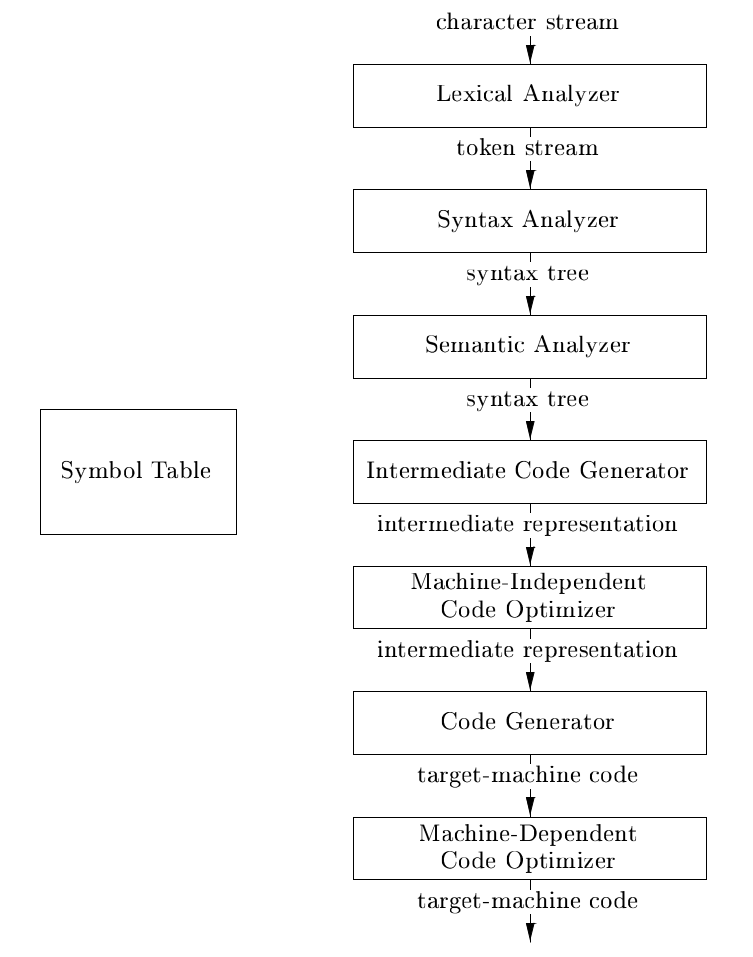
\includegraphics[scale=0.40]{compiler-phases.png}
    \caption{Phases of a compiler.}
    \label{fig:compiler-phases}
\end{figure}

In practice, phases might have unclear boundaries.
They can overlap and some may be skipped entirely.
In later sections, we will study the architecture of the Rust compiler \emph{rustc}
and explain its general architecture.

\end{document}
% !TeX root = ../../Thesis.tex
\documentclass[../../Thesis.tex]{subfiles}
\graphicspath{{\subfix{../../images/}}}

\begin{document}

\section{Model checking}

Model checking is a technique used in software development
to formally verify the correctness of a system's behavior
with respect to its specifications or requirements.
It involves constructing a mathematical model of the system
and analyzing it to ensure that it meets certain properties,
such as mutual exclusion when accessing shared resources,
absence of data races and deadlock-freedom.

The process of model checking begins by constructing a finite-state model of the system,
typically using a formal language, in the case of this work the language of Petri nets.
The model captures the system's behavior and the properties that are to be verified.
The next step is to perform an exhaustive search of the state space of the model
to ensure that all possible behaviors have been considered.
This search can be performed automatically using specialized software tools.

During the search, the model checker looks for counterexamples,
which are sequences of events that violate the system's specifications.
If a counterexample is found, the model checker provides information
on the state of the system at the time of the violation,
helping developers to identify and fix the problem.

Model checking has become an important technique
in the development of critical software systems,
such as aerospace \cite{carreno2005safety,monzon2009deadlock}
and automotive control systems \cite{Perronnet2019},
medical devices, and financial systems.
By verifying the correctness of the software before it is deployed,
developers can ensure that the system meets its requirements and is safe to use.

One of the main advantages of model checking is
that it provides a formal and rigorous approach to verifying software correctness.
Unlike traditional testing methods, which can only demonstrate the presence of errors,
model checking can prove the absence of errors.
This is particularly important for safety-critical systems like the ones mentioned before,
where a single error can have catastrophic consequences for human lives.
Model checking can also be automated, allowing developers to quickly
and efficiently verify the correctness of complex software systems.
This reduces the time and cost of software development
and increases confidence in the correctness of the system.

It is known that formal software verification tools are currently applied
in a few very specific fields where
formal proof of the correctness of the system is required.
\cite{reid:hatra:2020} discusses the importance of bringing verification
tools closer to developers through an approach
that seeks to maximize the cost-benefit ratio of its use.
Improvements in the usability of existing tools and
approaches to incorporate their use into the developer's routine are presented.
The paper starts from the premise that from the developer's point of view,
verification can be seen as a different type of unit or integration test.
Therefore, it is of utmost importance that running the verification is as easy as possible
and feedback is provided to the developer promptly during the development process
to increase adoption.

The main conclusion from this section is
that model checking could bring substantial improvements
to the table in terms of increased safety and reliability of software systems.
These objectives align with the goals of
the Rust programming language and the goals of this work.
Detecting deadlocks and missed signals in the source code at compile time could
help developers prevent hard-to-find bugs and get quick feedback on the correct use
of synchronization primitives, saving time and thus money in the development process.
One particular goal of this work is
to make the tool user-friendly and easy to get started with
so that its adoption benefits the larger community of Rust developers.

\end{document}

\chapter{State of the Art}
In this chapter, the literature on formal verification of Rust code
and Petri net modeling for deadlock detection is briefly reviewed.
Some of these previous publications contain approaches
that have guided this work.

In the next two sections, we will look at the existing tools,
their scope and their goals compared to the tool developed in this thesis.

Afterward, a survey of the existing Petri net libraries in the Rust ecosystem
as of early 2023 is provided to justify the need to implement a library
from the ground up.

As the next step, we explore the research community behind the \acrfull{MCC}
and the model checkers that participate in it
to confirm the potential of these tools
to analyze Petri net models of significant size.
This is relevant since the model checker acts
as the backend to the tool developed in this work.

Finally, three of the existing file formats for exchanging Petri nets are presented
and their purpose in the context of this work is explained.
\section{Formal verification of Rust code}

There are numerous automatic verification tools available for Rust code.
A recommended first approximation to the topic is
the survey produced by Alastair Reid, a researcher at Intel.
It explicitly lists that most formal verification tools
do not support concurrency \cite{reid2021}.

The \emph{Miri}\footnote{\url{https://github.com/rust-lang/miri}} interpreter
developed by the Rust project on GitHub is an experimental interpreter
for the intermediate representation of the Rust language
(Mid-level Intermediate Representation, commonly known as ``\acrshort{MIR}'')
that allows executing standard cargo project binaries
in a granularized way, instruction by instruction,
to check for the absence of \acrfull{UB}
and other errors in memory handling.
It detects memory leaks, unaligned memory accesses, data races,
and precondition or invariant violations in code marked as \texttt{unsafe}.

\cite{toman2015crust} introduces a formal checker for Rust
that does not require modifications to the source code.
It was tested on past versions of modules from the Rust standard library.
As a result, errors were detected in the use of memory in unsafe Rust code
which in reality took months to be discovered manually by the development team.
This exemplifies the importance of using automatic verification tools
to complement manual code reviews.

\cite{kani2023} is another well-known tool for the formal verification of Rust code
aimed at checking the \texttt{unsafe} blocks on a bit level.
It offers a proof harness analogous to the test harness provided by Rust.
Additionally, a plugin for cargo and VS Code is available.

As the documentation in the repository explains\footnote{\url{https://github.com/model-checking/kani}}, Kani verifies (among others):

\begin{itemize}
  \item Memory safety (e.g., null pointer dereferences)
  \item User-specified assertions (i.e., \Rustinline{assert!(...)})
  \item The absence of panics (e.g., \Rustinline{unwrap()} on \Rustinline{None} values)
  \item The absence of some types of unexpected behavior (e.g., arithmetic overflows)
\end{itemize}

However, concurrent programs are currently out of scope\footnote{\url{https://model-checking.github.io/kani/rust-feature-support.html}}.
The bottom line is that Kani offers an easy-to-use \acrshort{CLI} and a proof harness
that seamlessly integrate with the development process.
It serves as an illustration of the capabilities of model checking in modern software development.
\section{Deadlock detection using Petri nets}

Deadlock prevention is one of the classic strategies
to address this fundamental problem in concurrent programming,
as discussed in Sec. \ref{sec:deadlock-strategies}.
The main problem with the approach of detecting deadlocks before they occur
is proving that the desired type of deadlock is detected in all cases
and that no false negatives are produced in the process.
The Petri net-based approach, being a formal method, satisfies these conditions.
However, the difficulty of adoption lies mainly in the practicability of the solution
due to the large number of possible states in a real software project.

In \cite{karatkevich2014deadlock}, a method is proposed
to reduce the number of explored states
during the detection of deadlocks using reachability analysis.
These heuristics help improve the performance of the Petri net-based approach.
Another optimization is presented in \cite{kungas2005petri}.
The author proposes a very promising polynomial order method to avoid the problem
of the state explosion that underlies the naïve deadlock detection algorithm.
Through an algorithm that abstracts a given Petri net to a simpler representation,
a hierarchy of networks of increasing size is obtained
for which the verification of the absence of deadlocks is substantially faster.
It is, crudely put, a ``divide and conquer'' strategy
that checks for the absence of deadlocks in parts of the network
to later build the verification of the final whole
by adding parts to the initial small network.

Despite the previously mentioned caveats,
the use of Petri nets as a formal software verification method
has been established since the late 1980s.
Petri nets allow for intuitive modeling of synchronization primitives,
such as sending a message or waiting for the reception of a message.
Examples of these simple nets with correspondingly simple behavior
are found in \cite{heiner1992petri}.
These nets are construction blocks that can be combined to form a more complex system.

To put these models to use, there are two possibilities:

\begin{itemize}
      \item One is designing the system in terms of Petri nets
            and then translating the Petri nets to the source code.
      \item The other one is to translate the existing source code to a Petri net representation
            and then verify that the Petri net model satisfies the desired properties.
\end{itemize}

For the purposes of this work, we are interested in the latter.
This approach is not novel.
It has been implemented for other programming languages like C and Rust already,
as seen in the literature.

In \cite{kavi2002modeling} and \cite{moshtaghi2001},
a translation of some synchronization primitives available as part of
the POSIX library of threads (\texttt{pthread}) in C to Petri nets is described.
In particular, the translation supports:

\begin{itemize}
      \item The creation of threads with the function \texttt{pthread\_create}
            and the handling of the variable of type \texttt{pthread\_t}.
      \item The thread join operation with the \texttt{pthread\_join} function.
      \item The operation of acquiring a mutex with \texttt{pthread\_mutex\_lock}
            and its eventual manual release with \texttt{pthread\_mutex\_unlock}.
      \item The \texttt{pthread\_cond\_wait} and \texttt{pthread\_cond\_signal} functions
            for working with condition variables.
\end{itemize}

The source code for this library named ``C2Petri'' is disappointingly not found online,
as the publications are fairly old.

In a more recent master's thesis, \cite{meyer2020} establishes
the bases for a Petri net semantic for the Rust programming language.
He focuses his efforts however on single-threaded code,
limiting himself to the detection of deadlocks caused by
executing the \texttt{lock} operation twice on the same mutex in the main thread.
Unfortunately, the code available on GitHub\footnote{\url{https://github.com/Skasselbard/Granite}}
as part of the thesis is no longer valid for the new version of \emph{rustc}
since the internals of the compiler changed significantly in the last three years.

In a late 2022 pre-print, \cite{zhang2022deadlocks} implement a translation
of Rust source code to Petri nets for checking deadlocks.
The translation focuses on deadlocks caused by two types of locks
in the standard library: \texttt{std::sync::Mutex} and \texttt{std::sync::RwLock}.
The resulting Petri net is expressed in the \acrfull{PNML}
and fed into the model checker \acrfull{PIPE2}\footnote{\url{https://pipe2.sourceforge.net/}}
to perform reachability analysis.
Function calls are handled in a very different way compared to this work and
missed signals are not modeled at all.
The source code of their tool, named TRustPN, is not publicly available as of this writing.
Despite these limitations, the authors offer a very detailed and up-to-date survey
of static analysis tools for checking Rust code,
which could be appealing to the interested reader.
Moreover, they list several papers dedicated to
formalizing the semantics of the Rust programming language,
which are out of the scope of this work.
% !TeX root = ../../Thesis.tex
\documentclass[../../Thesis.tex]{subfiles}
\graphicspath{{\subfix{../../images/}}}

\begin{document}

\section{Petri nets libraries in Rust}

As part of the development of the translation of the source code to a Petri net,
it is necessary to use a Petri net library for the Rust programming language.
A quick search of the packages available on
\emph{crates.io}\footnote{\url{https://crates.io/}}, GitHub, and GitLab
revealed that there is, unfortunately, no well-maintained library.

Some Petri net simulators were found such as:

\begin{itemize}
    \item pns\footnote{\url{https://gitlab.com/porky11/pns}}:
          Programmed in C. It does not offer the option
          to export the resulting network to a standard format.
    \item PetriSim\footnote{\url{https://staff.um.edu.mt/jskl1/petrisim/index.html}}:
          An old DOS/PC simulator programmed in Bordland Pascal.
    \item WOLFGANG\footnote{\url{https://github.com/iig-uni-freiburg/WOLFGANG}}:
          A Petri net editor in Java, maintained by the Department of Computer Science
          at the University of Freiburg, Germany.
\end{itemize}

Regrettably, none of them meet the requirements of the task.

Since a Petri net is a graph, the possibility
of using a graph library and modifying it to suit the objectives of this work was considered.
Two graph libraries were found in Rust:

\begin{itemize}
    \item petgraph\footnote{\url{https://docs.rs/petgraph/latest/petgraph/}}:
          The most widely used library for graphs in \textit{crates.io}.
          It offers an option to export to the DOT format.
    \item gamma\footnote{\url{https://github.com/metamolecular/gamma}}:
          Unstable and unchanged since 2021. It does not offer the ability to export the graph.
\end{itemize}

None of the possibilities satisfies the requirement
to export the resulting network to the \acrshort{PNML} format.
In addition, if a graph library is used,
the operations of a Petri net should be implemented as a \emph{wrapper} around a graph,
which reduces the possibility of optimizations for our use case
and hinders the long-term extensibility of the project.

In conclusion, it is imperative
to implement a Petri net library in Rust from scratch as a separate project.
This contributes one more tool to the community that could be reused in the future.

\end{document}
\section{Exchange file formats for Petri nets}

As observed in the preceding chapter,
Petri nets are a widely used tool for modeling software systems.
However, due to the different classes of Petri nets
(simple Petri nets, high-level Petri nets, timed Petri nets,
stochastic Petri nets, colored Petri nets, to name a few),
designing a standardized exchange file format
compatible with all applications has proven challenging.
One reason for this is that
Petri nets can be implemented and represented in multiple ways,
depending on the specific objectives, given that they are a type of graph.

In order to guarantee a certain degree of interoperability between the tool developed
as part of this thesis and other existing and future tools, it is crucial
to investigate which file formats would be more convenient to support.
The aim is to support file formats that are suited to analysis as well as visualization,
allowing for the possibility of extension to additional formats in the future,
via a well-defined API in the Petri net library.
A literature review led to three relevant file formats that are presented next.

\subsection{Petri Net Markup Language}

The \acrfull{PNML}\footnote{\url{https://www.pnml.org/}}
is a standard file format designed
for the exchange of Petri nets
among different tools and software applications.
Its development was initiated
at the `Meeting on XML/SGML based Interchange Formats for Petri Nets'
held in Aarhus in June 2000 \cite{jungel2000petri,weber2003petri},
with the goal of providing
a standardized and widely accepted format for Petri net models.
PNML is an ISO standard consisting, as of 2023, of three parts:

\begin{itemize}
      \item ISO/IEC 15909-1:2004\footnote{\url{https://www.iso.org/standard/38225.html}}
            (and its latest revision ISO/IEC 15909-1:2019\footnote{\url{https://www.iso.org/standard/67235.html}})
            for concepts, definitions, and graphical notation.
      \item ISO/IEC 15909-2:2011\footnote{\url{https://www.iso.org/standard/43538.html}}
            for defining a transfer format based on XML.
      \item ISO/IEC 15909-3:2021\footnote{\url{https://www.iso.org/standard/81504.html}}
            for the extensions and structuring mechanisms.
\end{itemize}

It has become a de-facto standard
for exchanging Petri net models across different tools and systems.
It resulted from many years of hard work
to unify the notation as discussed in \cite{hillah:hal-01176335}.

\acrshort{PNML} has been designed to be a flexible and extensible format
that can represent different classes of Petri nets,
including simple Petri nets and high-level Petri nets.
It is based on the \acrfull{XML}
which makes it easy to read and parse by humans and machines alike.
Additionally, \acrshort{PNML} supports the use of metadata
to provide additional information about the Petri net models,
such as authorship, date of creation, and licensing information.

The development of \acrshort{PNML} has significantly improved
the interoperability and exchange of Petri net models
among different tools and systems.
Before the adoption of \acrshort{PNML},
exchanging Petri net models was a challenging task,
as different tools used proprietary formats
that were often incompatible with each other.
\acrshort{PNML} has greatly simplified this process,
enabling researchers and practitioners
to share and collaborate on Petri net models with ease.
Its use has also facilitated the development of new tools
and software applications for Petri nets,
as it provides a standard format
that can be easily parsed and processed by different systems.
For instance, it is the format used
in \cite{zhang2022deadlocks} and it is supported in \cite{meyer2020}.

\subsection{GraphViz DOT format}

The DOT format is a graph description language
used for creating visual representations of graphs and networks,
which is part of the open-source GraphViz suite\footnote{\url{https://graphviz.org/}}.
It was created in the early 1990s at AT\&T Labs Research
as a simple, concise, and human-readable language for describing graphs.
The GraphViz suite provides several tools for working with DOT files,
including the ability to automatically generate layouts for complex graphs and
to export visualizations in a range of formats, including PNG, PDF, and SVG.

DOT can be used to represent Petri nets in a graphical format, which makes it easy
to visualize the structure and behavior of the system being modeled.
It is particularly useful for visualizing large Petri nets,
as the user can navigate through the image
to gain an understanding of how the tokens flow through the net.

The DOT format is text-based and easy to use,
making it a popular choice for generating visual representations of graphs.
This simplicity also means that DOT files can be easily generated by programs
and can be read by a wide range of software tools,
which is essential for interoperability.
Additionally, DOT allows for the specification of various graph properties,
such as node shapes, colors, and styles \cite{dot2015},
which can be used to represent different aspects of a Petri net,
such as places, transitions, and arcs.
This flexibility in specifying visual properties also enables users
to customize the visualization to their needs and
to highlight particular features of the Petri net
that are important for their analysis.

\subsection{LoLA - Low Level Petri Net Analyzer}

\acrfull{LoLA} is a state-of-the-art model checker
developed at the University of Rostock in
Germany\footnote{\url{https://theo.informatik.uni-rostock.de/theo-forschung/tools/lola/}}
and published under the GNU Affero General Public License.
\acrshort{LoLA} is a tool that can check
if a system satisfies a given property expressed in \acrfull{CTL*}.
Its particular strength is the evaluation of simple properties
such as deadlock freedom or reachability as stated on the website.

This is the model checker used in \cite{meyer2020} and in this work.
Therefore, it is necessary to implement the file format required by the tool.
Examples are presented in Sec. \ref{sec:integration-tests}.

\chapter{Design of the proposed solution}
Now that the relevant background topics have been covered,
we can proceed to delve into the specifics of the design of the translation process.
The design is marked by three crucial architectural choices
that will be elaborated on in this chapter:

\begin{enumerate}
    \item The decision to utilize the Rust compiler as a backend for the translation.
    \item Basing the translation on the \acrfull{MIR}.
    \item Inlining function calls in the Petri net.
\end{enumerate}

Throughout this chapter,
we will conduct an in-depth analysis
of the Rust compiler's internal mechanisms and its relevant compilation stages.
\section{In search of a backend}

To put it succinctly, two approaches for translating Rust code to Petri nets exist.
The first option is to create a translator from scratch,
while the second option is to build upon an existing tool.

The first option may seem attractive at first,
considering that it gives the developer
the freedom to shape the tool according to his/her desires.
Features can be added as required and
data structures can be tailored to the specific purpose.
Nonetheless, this flexibility comes at a high price.
In order to support a reasonable subset of the Rust programming language,
substantial amounts of effort need to be invested into the task.
Complex language constructs, such as macros, generics, or the rich type system itself,
must be comprehended in their most intricate details to be translated effectively.
The result is, essentially, a new compiler for Rust code.
Noting that the Rust compiler was developed over many years and
with the support of a large community of contributors,
it becomes clear that this path is nothing more than work duplication.
It is indeed a Herculean labor that would require the full-time dedication of a whole team
to maintain and keep up-to-date with the newest changes in the Rust language and the compiler.

On the other hand, there is the possibility
of integrating with the existing Rust compiler,
which is available under an open-source license
and its documentation is extensive and regularly updated.
This frees the implementation partly from having to deal with the changes to the language,
giving more time to focus on the features that add value to the users.
Hence the compiler plays the role of a backend on which the static analysis relies.
Of course, this requires learning the compiler internals
but this is not the first time that a tool sets off to do this.
For instance, the official Rust linter,
\emph{clippy}\footnote{\url{https://github.com/rust-lang/rust-clippy}},
analyzes the Rust code for incorrect, inefficient, or non-idiomatic constructs.
It is an extremely valuable tool for developers that goes beyond the standard checks
performed during compilation.

Supporting all the language features from the beginning
and collaborating with the community is key to the success of the proposed solution.
Therefore, it is advisable to integrate with the existing ecosystem
and reuse as much work as possible.
Due to the above reasons, this project is based on \emph{rustc}.
We will now study the relevant parts of the Rust compiler in more detail.
\section{Rust compiler: \emph{rustc}}
\label{sec:rustc}

The Rust compiler, \emph{rustc}, is responsible for translating Rust code into executable code.
However, \emph{rustc} is not a traditional compiler in the sense
that it performs multiple passes over the code,
as described in Sec. \ref{sec:compiler-architecture}.
Instead, \emph{rustc} is built on a query-based system that supports incremental compilation.

In \emph{rustc}'s query system, the compiler computes a dependency graph between code artifacts,
including source files, crates, and intermediate artifacts, such as object files.
The query system then uses this graph to efficiently recompile
only those artifacts that have changed since the last
compilation\footnote{\url{https://rustc-dev-guide.rust-lang.org/queries/incremental-compilation.html}}.
This incremental compilation can significantly
reduce the compilation time for large projects,
making it easier to develop and iterate on Rust code.

The query system also enables the Rust compiler to perform other optimizations,
such as memoization and caching of intermediate results.
For example, if a function's return value has been computed before,
the query system can return the cached result instead of recomputing it,
further reducing compilation time.

Another important design choice in \emph{rustc} is interning.
Interning is a technique to store strings and
other data structures in a memory-efficient way.
Instead of storing multiple copies of the same string or data structure,
the Rust compiler stores only one copy in a special allocator called an \emph{arena}.
References to values stored in the arena are passed around between different parts
of the compiler and they can be compared cheaply by comparing pointers.
This can reduce memory usage and speed up operations
that compare or manipulate strings and data structures.

\emph{rustc} uses the LLVM compiler infrastructure\footnote{\url{https://llvm.org/}}
to perform low-level code generation and optimization.
LLVM provides a flexible framework for compiling code
to a variety of targets, including native machine code and \acrfull{WASM}.
The Rust compiler uses LLVM to optimize code for performance and
to generate high-quality code for a variety of platforms.
Instead of generating machine code, it only needs
to generate the source code's LLVM \acrfull{IR}
and then instruct LLVM to transform this to the compilation target,
applying the desired optimizations.

\emph{rustc} is programmed in Rust.
In order to compile the newer version of the compiler
and the newer standard library version that goes with it,
a slightly older version of \emph{rustc} and the standard library is used.
This process is called \emph{bootstrapping} and it implies
that one of the major users of Rust is the Rust compiler itself.
Considering that a new stable version is released every six weeks,
bootstrapping involves a substantial amount of complexity and is described in detail
in the documentation\footnote{\url{https://rustc-dev-guide.rust-lang.org/building/bootstrapping.html}}
and in conferences \cite{nelson2022} and tutorials \cite{klock2022} by members of the Rust team.

\subsection{Compilation stages}

The existence of the query system does not imply
that \emph{rustc} does not have compilation phases at all.
On the contrary, several stages of compilation are required
to transform Rust source code into machine code that can be executed on a computer.
These stages involve multiple intermediate representations of the program,
each one optimized for a specific purpose.
We will now briefly describe these stages.
A more complete overview is found
in the documentation\footnote{\url{https://rustc-dev-guide.rust-lang.org/overview.html}}.

\subsubsection{Lexing and parsing}

First, the raw Rust source text is analyzed by a low-level lexer.
At this stage, the source text is turned
into a stream of atomic source code units known as tokens.

Then parsing takes place.
The stream of tokens is converted into an \acrshort{AST}.
Interning of string values occurs here.
Macro expansion, \acrshort{AST} validation,
name resolution, and early linting also take place during this stage.
The resulting intermediate representation from this step is thus the \acrshort{AST}.

\subsubsection{HIR lowering}

Next, the \acrshort{AST} is converted to \acrfull{HIR}.
This process is known as ``lowering''.
This representation looks like Rust code but with complex constructs desugared
to simpler versions.
For instance, all \texttt{while} and \texttt{for} loops are converted into simpler
\texttt{loop} loops.

The \acrshort{HIR} is used to perform some important steps:

\begin{enumerate}
      \item \emph{type inference}: The automatic detection of a type
            of an expression, e.g. when declaring variables with \texttt{let}.
      \item \emph{trait solving}: Ensuring that each implementation block (\texttt{impl})
            refers to a valid, existing trait.
      \item \emph{type checking}: This process converts the types written by the user
            into the internal representation used by the compiler.
            It is, in other words, where types are interned.
            Then, using this information, the type safety, correctness, and coherence are verified.
\end{enumerate}

\subsubsection{MIR lowering}

In this stage, the \acrshort{HIR} is lowered to \acrfull{MIR},
which is used for \emph{borrow checking}.
As part of the process, the \acrfull{THIR} is constructed,
which is a representation that is easier to convert to \acrshort{MIR} than the \acrshort{HIR}.

The \acrshort{THIR} is an even more desugared version of \acrshort{HIR}.
It is used for pattern and exhaustiveness matching.
It is similar to the \acrshort{HIR}, but with all types and method calls made explicit.
Furthermore, implicit dereferences are included where needed.

Many optimizations are performed on the \acrshort{MIR}
as it is still a very generic representation.
Optimizations are in some cases easier
to perform on the \acrshort{MIR} than on the subsequent LLVM \acrshort{IR}.

\subsubsection{Code generation}

This is the last stage when producing a binary.
It includes the call to LLVM for code generation
and the corresponding optimizations.
To this effect, the \acrshort{MIR} is converted to LLVM \acrshort{IR}.

LLVM \acrshort{IR} is the standard form of input for the LLVM compiler
that all compilers using LLVM, such as the \emph{clang} C compiler, utilize.
It is a type of assembly language that is well-annotated
and designed to be easy for other compilers to produce.
Additionally, it is designed to be rich enough to enable LLVM
to perform several optimizations on it.

LLVM transforms the LLVM \acrshort{IR} to machine code
and applies many more optimizations.
Finally, the object files with assembly code in them may be
linked together to form the binary.

\subsection{Rust nightly}
\label{sec:rust-nightly}

Understanding the release model of Rust is crucial
for the successful implementation of the tool proposed in this work.
The reason is that to use the crates of \emph{rustc} as a dependency in our project,
it must be compiled with the \emph{nightly} version.

The nightly Rust compiler refers to a specific build of \emph{rustc}
that is updated every night with the latest changes and improvements
but also includes experimental or unstable features that are not yet part of the stable release.
In Rust, the language and its standard library are versioned using a ``release train'' model,
where there are three main release channels:
stable, beta, and nightly\footnote{\url{https://forge.rust-lang.org/}}.

The stable release of the Rust compiler is
the most widely used and recommended version for production use.
It goes through a rigorous testing and stabilization process
to ensure that it provides a stable and reliable experience for developers.
The stable release only includes features and improvements
that have been thoroughly reviewed, tested, and deemed stable enough for production use.

On the other hand, the nightly Rust compiler is the most bleeding-edge version,
where new features, bug fixes, and experimental changes are introduced on a daily basis.
It is used by Rust language developers and contributors for testing and development purposes
but it is not recommended for production use
due to the potential instability and lack of long-term support.

Each feature exclusive to the nightly version is behind a so-called \emph{feature flag}.
They may only be used when compiling with the nightly toolchain.
Features flags may enable

\begin{itemize}
      \item syntactic constructs that are not available on the stable version,
      \item library functions exclusive to the nightly version,
      \item support for specific hardware instructions of a given \acrshort{ISA} or platform,
      \item additional compiler flags.
\end{itemize}

The full list of feature flags is found in \cite{unstable-book}
and contains more than 500 entries in total.
In a more concise manner, the Rust language used inside of \emph{rustc} is
a superset of the stable Rust language used outside of it.
These differences should be taken into account
when working on the compiler or building software that directly depends on the compiler.
% !TeX root = ../Thesis.tex
\documentclass[../Thesis.tex]{subfiles}
\graphicspath{{\subfix{../images/}}}

\begin{document}

\section[Interception strategy]
 {Interception strategy:\\Selecting a suitable starting point for the translation}
\label{sec:interception-strategy}

In this section, a rationale for selecting the \acrfull{MIR}
as the starting point for the translation to a Petri net is elucidated.
This architectural design choice is justified for several reasons.

\subsection{Benefits}

First, the \acrshort{MIR} is
the lowest machine-independent \acrshort{IR} used in \emph{rustc}.
It captures the semantics of Rust code
after it has undergone a series of optimization passes
without relying on the details of any particular machine.
By intercepting the translation at this stage,
the static analysis tool leverages the benefits of these optimizations,
such as constant folding, dead code elimination, and inlining,
which results in a more efficient and overall smaller Petri net representation.

Second, intercepting the compilation after the previous stages are completed
offers an advantage in terms of efficiency and code reuse.
By this stage, the Rust compiler has already performed crucial steps
such as borrow checking, type checking,
monomorphization of generic code, and macro expansion, among others.
These steps are resource-intensive
and involve complex analysis of the Rust code to ensure correctness and safety.
Re-implementing these steps in our tool from scratch
would be redundant and time-consuming.
It would require duplicating the efforts of the Rust compiler
and may introduce potential inconsistencies or errors.
By building on top of the existing \acrshort{MIR},
we take advantage of the work already done by \emph{rustc}.
This not only saves effort but also ensures that our static analysis tool
is aligned with the same level of correctness and safety as the Rust compiler.

Third, it simplifies the maintenance task of staying up-to-date
with the ongoing additions to the Rust language and its compiler.
Rust is a fast-evolving language and its compiler is
constantly updated with new features, bug fixes, and performance optimizations.
Repurposing the \acrshort{MIR} means our tool can benefit from these updates
without having to independently implement and maintain those changes.
This provides overall a more robust and reliable static analysis solution.

Furthermore, as it will be explained in the next section, the \acrshort{MIR}
is based on the concept of a \acrfull{CFG}, i.e. a type of graph found in compilers.
That means that \acrshort{MIR} and Petri nets are both graph representations,
which makes the \acrshort{MIR} particularly amenable to translation.
Both \acrshort{MIR} and Petri nets can be seen as graphical models
that capture the relationships and interactions between different entities.
The \acrshort{MIR} graph represents the underlying execution flow within a Rust program,
while a Petri net captures the state transitions and event occurrences in a system.
Therefore, it becomes easier to convert the \acrshort{MIR} to a Petri net,
as the graph structure and relationships are already present.
This allows for a more straightforward and efficient translation process
without having to create a graph structure from thin air,
resulting in better integration between the \acrshort{MIR}
and the Petri net model for deadlock detection.

Finally, working with the \acrshort{MIR} synergizes
with incremental compilation and modular analysis.
In fact, one of the reasons why \acrshort{MIR} was introduced
in the first place was incremental compilation \cite{matsakis2016mir}.
Even though it is not mandatory in the initial implementation,
the tool could profit from incremental compilation
and perform analysis on a per-crate/per-module basis,
allowing for faster and more efficient analysis of large Rust codebases.

\subsection{Limitations}

There are however some limitations to the approach of basing the translation
on the \acrfull{MIR}.

The most important one is that the \acrshort{MIR} is subject to change.
No stability guarantees are made in terms of
how the Rust code will be translated to \acrshort{MIR}
or which its constituent elements \acrshort{MIR} are.
These are internal details that the compiler developers reserve for themselves.
In short, \acrshort{MIR} as an interface is not stable.
As work on the compiler continues,
the \acrshort{MIR} undergoes modifications
to incorporate new language features, optimizations, or bug fixes,
which may require frequent updates and adjustments to the translation process,
increasing the maintenance cost.

In the course of this project, this situation occurred numerous times.
As an example, in the period between mid-February 2023 and mid-April 2023,
the code was modified 7 times to accommodate these changes.
They were always a few lines of code in size and detected by tests.
We will discuss how tests play a significant role
in coping with these changes in Sec. \ref{sec:integration-tests}.

On the same note, \cite{meyer2020} also relied on the \acrshort{MIR}
but did not incorporate tests to deal with the newer nightly versions.
As a result, the toolchain was pinned to an exact nightly
version\footnote{\url{https://github.com/Skasselbard/Granite/blob/master/rust-toolchain}}
to prevent the implementation from breaking before the publication of the thesis.

Another drawback worth mentioning is that, in some instances,
generic code could take the form of a function whose behavior can be modeled
by the same Petri net in all cases.
Under these circumstances, the \acrshort{MIR} could be ``condensed'' further
before translating it to a Petri net.
Similarly, some parts of the \acrshort{MIR} may be superfluous
to the deadlock detection analysis and its translation may enlarge the output,
which slows down the reachability analysis done by the model checker.
This can be countered with careful optimizations,
which will be proposed in Chapter \ref{chap:future-work}.

\subsection{Synthesis}

In conclusion, despite the drawbacks mentioned earlier,
intercepting the translation at the \acrshort{MIR} level offers significant advantages,
including maximizing the utilization of the existing compiler code,
reducing the implementation effort, and a more natural mapping to Petri nets.
These benefits outweigh the cons and make the \acrshort{MIR}
a compelling starting point for the translation
in the context of building a static analysis tool
for detecting deadlocks and missed signals in Rust code.

Both \cite{meyer2020} and \cite{zhang2022deadlocks} base their translations
on the \acrshort{MIR} as well and to the best knowledge of this author, there is
no analogous tool that performed a translation to Petri nets
starting from a higher-level \acrshort{IR}.

\end{document}
% !TeX root = ../../Thesis.tex
\documentclass[../../Thesis.tex]{subfiles}
\graphicspath{{\subfix{../../images/}}}

\begin{document}

\section{Mid-level Intermediate Representation (MIR)}

An overview of the \acrfull{MIR} is provided in this section.
\acrshort{MIR} was introduced in
RFC 1211\footnote{\url{https://rust-lang.github.io/rfcs/1211-mir.html}}
in August 2015.
We will explore its different parts,
how different code fragments are mapped to them,
and the underlying graph structure.

\begin{listing}
    \begin{minted}{Rust}
        fn main() {
            match std::env::args().len() {
                1 => 2,
                3 => 6,
                _ => 0,
            };
        }
    \end{minted}
    \caption{Simple Rust program to explain the MIR components.}
    \label{lst:rust-code-example}
\end{listing}

\begin{longlisting}
    \begin{minted}{Rust}
        // WARNING: This output format is intended for human consumers only
        // and is subject to change without notice. Knock yourself out.
        fn main() -> () {
            let mut _0: ();               // return place in scope 0 at src/main.rs:1:11: 1:11
            let mut _1: usize;            // in scope 0 at src/main.rs:2:11: 2:33
            let mut _2: &std::env::Args;  // in scope 0 at src/main.rs:2:11: 2:33
            let _3: std::env::Args;       // in scope 0 at src/main.rs:2:11: 2:27

            bb0: {
                _3 = args() -> bb1;       // scope 0 at src/main.rs:2:11: 2:27
                                          // mir::Constant
                                          // + span: src/main.rs:2:11: 2:25
                                          // + literal: Const { ty: fn() ->
                                          //   Args {args}, val: Value(<ZST>) }
            }

            bb1: {
                _2 = &_3;                 // scope 0 at src/main.rs:2:11: 2:33
                _1 = <Args as ExactSizeIterator>::len(move _2) -> [return: bb2, unwind: bb4];
                                          // scope 0 at src/main.rs:2:11: 2:33
                                          // mir::Constant
                                          // + span: src/main.rs:2:28: 2:31
                                          // + literal: Const { ty: for<'a> fn(&'a Args) ->
                                          //   usize {<Args as ExactSizeIterator>::len},
                                          //   val: Value(<ZST>) }
            }

            bb2: {
                drop(_3) -> bb3;          // scope 0 at src/main.rs:6:6: 6:7
            }

            bb3: {
                return;                   // scope 0 at src/main.rs:7:2: 7:2
            }

            bb4 (cleanup): {
                drop(_3) -> [return: bb5, unwind terminate]; // scope 0 at src/main.rs:6:6: 6:7
            }

            bb5 (cleanup): {
                resume;                   // scope 0 at src/main.rs:1:1: 7:2
            }
        }
    \end{minted}
    \caption{MIR of Listing \ref{lst:rust-code-example}
        compiled using rustc 1.71.0-nightly in debug mode.}
    \label{lst:mir-output-debug-example}
\end{longlisting}

Consider the example code listed in Listing \ref{lst:rust-code-example},
the corresponding \acrshort{MIR}\footnote{The comments in the MIR have been slightly modified to improve the output}
is shown in Listing \ref{lst:mir-output-debug-example}.
Notice the explicit warning at the top of the generated output.
It will be omitted in the subsequent listings for simplicity.
Moreover, output depends on the following factors:

\begin{itemize}
    \item The \emph{rustc} version in use,
          alternatively the release channel (stable, beta, or nightly).
    \item The build type: \emph{debug} or \emph{release}.
          By default, the command \texttt{cargo build} generates a \emph{debug} build,
          while \texttt{cargo build --release} produces a \emph{release} build.
\end{itemize}

To illustrate this variability, Listing \ref{lst:mir-output-release-example}
shows the output when compiling the same program in \emph{release} mode.
The distinguishing feature found in \emph{release} builds is
the presence of the \Rustinline{StorageLive} and \Rustinline{StorageDead} statements.
On the other hand, \emph{debug} builds generate
shorter and clearer \acrshort{MIR} that is closer to what the user wrote.
For this reason, unless otherwise stated,
the listings in this work contain \acrshort{MIR} generated in \emph{debug} builds.

\begin{longlisting}
    \begin{minted}{Rust}
        // WARNING: This output format is intended for human consumers only
        // and is subject to change without notice. Knock yourself out.
        fn main() -> () {
            let mut _0: ();               // return place in scope 0 at src/main.rs:1:11: 1:11
            let mut _1: usize;            // in scope 0 at src/main.rs:2:11: 2:33
            let mut _2: &std::env::Args;  // in scope 0 at src/main.rs:2:11: 2:33
            let _3: std::env::Args;       // in scope 0 at src/main.rs:2:11: 2:27

            bb0: {
                StorageLive(_1);          // scope 0 at src/main.rs:2:11: 2:33
                StorageLive(_2);          // scope 0 at src/main.rs:2:11: 2:33
                StorageLive(_3);          // scope 0 at src/main.rs:2:11: 2:27
                _3 = args() -> bb1;       // scope 0 at src/main.rs:2:11: 2:27
                                          // mir::Constant
                                          // + span: src/main.rs:2:11: 2:25
                                          // + literal: Const { ty: fn() ->
                                          //   Args {args},
                                          //   val: Value(<ZST>) }
            }

            bb1: {
                _2 = &_3;                 // scope 0 at src/main.rs:2:11: 2:33
                _1 = <Args as ExactSizeIterator>::len(move _2) -> [return: bb2, unwind: bb4];
                                          // scope 0 at src/main.rs:2:11: 2:33
                                          // mir::Constant
                                          // + span: src/main.rs:2:28: 2:31
                                          // + literal: Const { ty: for<'a> fn(&'a Args) ->
                                          //   usize {<Args as ExactSizeIterator>::len},
                                          //   val: Value(<ZST>) }
            }

            bb2: {
                StorageDead(_2);          // scope 0 at src/main.rs:2:32: 2:33
                drop(_3) -> bb3;          // scope 0 at src/main.rs:6:6: 6:7
            }

            bb3: {
                StorageDead(_3);          // scope 0 at src/main.rs:6:6: 6:7
                StorageDead(_1);          // scope 0 at src/main.rs:6:6: 6:7
                return;                   // scope 0 at src/main.rs:7:2: 7:2
            }

            bb4 (cleanup): {
                drop(_3) -> [return: bb5, unwind terminate]; // scope 0 at src/main.rs:6:6: 6:7
            }

            bb5 (cleanup): {
                resume;                   // scope 0 at src/main.rs:1:1: 7:2
            }
        }
    \end{minted}
    \caption{MIR of Listing \ref{lst:rust-code-example}
        compiled using rustc 1.71.0-nightly in release mode.}
    \label{lst:mir-output-release-example}
\end{longlisting}

The specific formatting when converting \acrshort{MIR} to a string has changed only slightly over time.
See \cite[Section 3.3]{meyer2020} for an example of older output from mid-2019.

As stated in Sec. \ref{sec:interception-strategy}, the \acrshort{MIR} is derived
from a previously existing \acrfull{CFG} in the Rust compiler.
Fundamentally, a \acrshort{CFG} is a graph representation of a program
that exposes the underlying control flow.

The MIR is formed by functions.
Each function is represented as a series of \acrfull{BB} connected by directed edges.
Each \acrshort{BB} contains zero or more \emph{statements} (usually abbreviated as ``STMT'')
and lastly one \emph{terminator statement}, for short \emph{terminator}.
The terminator is the only statement in which the program can issue an instruction
that directs the control flow to another basic block inside the same function
or to call another function.
Branching as in Rust's \Rustinline{match} or \Rustinline{if} statements can occur only in terminators.
Terminators play the role of mapping the high-level constructs
for conditional execution and looping to the low-level representation in machine code
as simple conditional or unconditional \Rustinline{branch} instructions.

In Fig. \ref{fig:mir-cfg-example}, the graph representation
for the MIR shown in Listing \ref{lst:mir-output-debug-example} is presented as an example.
The statements are colored in light blue and the terminators in light red.
To make the kind of terminator statement clearer,
extra annotations as in \texttt{CALL:} or \texttt{DROP:} were added.

\begin{figure}[!htb]
    \centering
    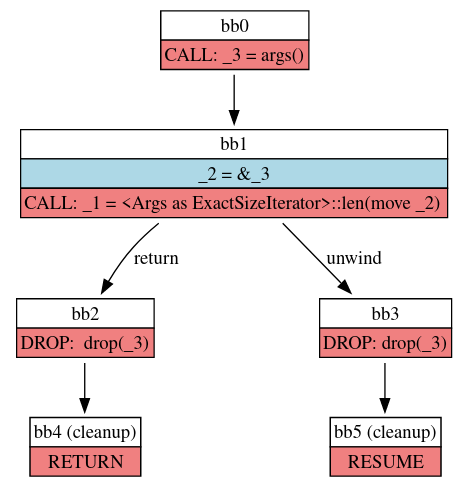
\includegraphics[scale=0.60]{mir-cfg-example.png}
    \caption{The control flow graph representation of the MIR shown in Listing \ref{lst:mir-output-debug-example}.}
    \label{fig:mir-cfg-example}
\end{figure}

It should be noted that the function call to \Rustinline{std::env::args().len()}
in Line 2 in Listing \ref{lst:rust-code-example} may return successfully or fail.
The latter triggers an unwinding of the stack, ending the program and reporting an error.
This is represented by the branching at the end of BB1 where the code execution
may take the left path or the right path down the graph.
The left branch (BB4 and BB5) corresponds to the correct execution of the program,
while the right branch relates to the abnormal termination of the program.

There are different kinds of terminators and these are specific to the Rust semantics.
We will introduce some of them to clarify the meaning of the example presented.

\begin{itemize}
    \item As expected, a terminator of type \texttt{CALL:} calls a function, which returns a value,
          and continues execution to the next \acrshort{BB}.
    \item A terminator of type \texttt{DROP:} frees up the memory of the variable passed in.
          It executes the destructors\footnote{\url{https://doc.rust-lang.org/stable/reference/destructors.html}}
          and performs all the necessary cleanup tasks.
          From that point on, the variable cannot be used anymore in the program.
    \item \texttt{RETURN:} returns from the function.
          The return value is always stored in the local variable \Rustinline{_0}, as we will see shortly.
    \item \texttt{RESUME:} indicates that the process should continue unwinding.
          Analogously to a return, this marks the end of this invocation of the function.
          It is only permitted in cleanup blocks.
\end{itemize}

The complete list of terminator kinds can be found in the nightly
documentation\footnote{\url{https://doc.rust-lang.org/stable/nightly-rustc/rustc_middle/mir/enum.TerminatorKind.html}}.
Other kinds of terminators will be discussed in detail in Sec. \ref{sec:terminators}.

Regarding the variables, the data in MIR can be divided into two categories:
\emph{locals} and \emph{places}.
It is critical to observe that these ``places'' are
\emph{not} related to the places in Petri nets.
Places are used to represent all types of memory locations (including aliases),
while locals are limited to stack-based memory locations
(i.e. local variables of a function).
In other words, places are more general and locals are a special case of a place,
therefore places are not always equivalent to locals.
Conveniently, all the places are also locals in Fig. \ref{fig:mir-cfg-example}.

Locals are identified by an increasing non-negative index
and are emitted by the compiler as a string of the form ``\Rustinline{_<index>}''.
In particular, the return value of the function
is always stored in the first local \Rustinline{_0}.
This matches closely the low-level representation on the stack.

\subsection{Step-by-step example}

In this subsection, we will give a short explanation of what happens
in each basic block of Fig. \ref{fig:mir-cfg-example}
to ensure that all necessary information is covered.
Moreover, this illustrates how the MIR output represents higher-level constructs
often encountered when programming in Rust.

\subsubsection{BB0}

\begin{itemize}
    \item The \Rustinline{main()} function starts at BB0.
    \item A function is called (\Rustinline{std::env::args()})
          to obtain an iterator over the arguments provided to the program.
    \item The return value of the function, the iterator,
          is assigned to the local \Rustinline{_3}.
    \item Execution continues in BB1.
\end{itemize}

\subsubsection{BB1}

\begin{itemize}
    \item A reference to the iterator stored in \Rustinline{_3} is generated
          and stored in the local \Rustinline{_2} (similar to the ``\&'' operator in C).
          This is necessary for calling methods
          because methods receive a reference
          to a struct of the same type (\Rustinline{&self}) as their first argument.
    \item The reference stored in \Rustinline{_2} is passed to
          the method \Rustinline{std::env::Args::len()} by moving
          and the function is called.
    \item The return value of the function,
          the number of arguments passed to the function, is assigned to the local \Rustinline{_1}.
    \item Execution continues in BB2 if successful, in BB4 in case of panic.
\end{itemize}

\subsubsection{BB2}

\begin{itemize}
    \item The variable \Rustinline{_3}, whose value is the iterator over the arguments,
          is \emph{dropped} since it is no longer needed.
    \item Execution continues in BB3.
\end{itemize}

\subsubsection{BB3}

\begin{itemize}
    \item The function returns.
          The return value (local \Rustinline{_0}) is of type "unit"\footnote{\url{https://doc.rust-lang.org/std/primitive.unit.html}},
          which is similar to a \texttt{void} function in C, i.e. it does not return anything.
          This is how \Rustinline{main()} was defined in Listing \ref{lst:rust-code-example}.
\end{itemize}

\subsubsection{BB4}

\begin{itemize}
    \item The variable \Rustinline{_3}, whose value is the iterator over the arguments,
          is \emph{dropped} since it is no longer needed.
    \item If the drop is successful, execution continues in BB5,
          otherwise terminate the program immediately.
\end{itemize}

\subsubsection{BB5}

\begin{itemize}
    \item Continue unwinding the stack.
          This is the standard protocol defined for handling catastrophic error cases
          that cannot be handled by the program.
          Implementation details can be found in the
          documentation\footnote{\url{https://rustc-dev-guide.rust-lang.org/panic-implementation.html}.}
\end{itemize}

\end{document}
\section{Function inlining in the translation to Petri nets}
\label{sec:function-inlining}

In this section, a thorough analysis and motivation for the third design decision
listed at the beginning of the chapter, namely inlining function calls, is presented.

Modeling functions in \acrshort{PN} is a crucial aspect of the translation
because it is the basic unit of the \acrshort{MIR}.
By representing the functions in the \acrshort{MIR} as \acrshort{PN} and connecting them accordingly,
the control flow and data shared between the threads in the program
can be captured in a formal framework.
Afterward, the Petri net is analyzed by a model checker
in order to identify potential deadlocks or lost signals.
This approach is especially useful when working with large and complex systems
that may have many interrelated threads and functions,
where the deadlock situation may not be evident even to an experienced code reviewer.

When translating \acrshort{MIR} functions to \acrshort{PN}, one key question that arises is
whether to reuse the same representation for every call to a specific function or
to ``inline'' the corresponding representation every time the function is called.
Expressed differently, each function maps to a subnet
in the final \acrshort{PN} obtained after the translation, i.e.,
a connected subgraph formed by the places and transitions
that model the behavior of the specific function.
This smaller part of the net can either be present only once in the \acrshort{PN}
and all calls to this function connect to it,
or be repeated for every instance of a call to the function in the Rust code.

Reusing the same model for every function seems at first glance more efficient,
as the \acrshort{PN} obtained is smaller.
However, this approach can also lead to invalid states
that were not present in the original Rust program.
These can be the source of false positives during deadlock detection,
as these extraneous states may violate
the safety guarantees offered by the compiler.

On the other hand, inlining the model every time a function is called results in
a larger \acrshort{PN}, which requires more memory and \acrshort{CPU} time to be analyzed,
but it can also improve the accuracy of the analysis by ensuring
that each function call is represented by a separate Petri net structure
that captures its specific data dependencies in the context
in which the function call occurs in the code.

\subsection{The basic case}

The impact of these subtle details can only
be fully comprehended with an appropriate example.
Therefore, consider first the most simple abstraction of a function call in
the language of Petri nets, formed by a single transition and
two places representing the start and end of the function.
This is seen in Fig. \ref{fig:simplest-function}.
The function call is treated as a black box,
all details are abstracted away in the transition.
We care only about where the function starts and where it ends.

\begin{figure}[!htb]
    \centering
    \includesvg[width=0.3\linewidth]{simplest-function.svg}
    \caption{The simplest Petri net model for a function call.}
    \label{fig:simplest-function}
\end{figure}

Observe now such a function in the context of a Rust program.
Listing \ref{lst:repeated-function-call} provides a simple example
in which one function is called
five times consecutively in a \Rustinline{for} loop.
A possible \acrshort{PN} that models the program
is found in Fig. \ref{fig:repeated-function-call}.
It should be emphasized that
this net and the subsequent ones in this section
do \emph{not} result from a translation of the MIR.
They are simplifications to showcase the difficulties
of dealing with functions called in various places in the code.

\begin{listing}[!htb]
    \begin{minted}{Rust}
        fn simple_function() {}

        pub fn main() {
            for n in 0..5 {
                simple_function();
            }
        }
    \end{minted}
    \caption{A simple Rust program with a repeated function call.}
    \label{lst:repeated-function-call}
\end{listing}

\begin{figure}[!htb]
    \centering
    \includesvg[width=0.7\linewidth]{repeated-function-call.svg}
    \caption{A possible \acrshort{PN} for the code in Listing \ref{lst:repeated-function-call}
        applying the model of Fig. \ref{fig:simplest-function}.}
    \label{fig:repeated-function-call}
\end{figure}

\subsection{A characterization of the problem}

The troublesome scenario has not emerged so far.
It manifests only when a function is called
in at least two different places in the code or,
in simpler terms, the expression \Rustinline{simple_function()} appears twice or more.
Listing \ref{lst:two-simple-function-calls} satisfies this condition
and is designed to exhibit
the extraneous behavior described at the beginning of the section.

\begin{listing}[!htb]
    \begin{minted}{Rust}
        fn simple_function() {}

        pub fn main() {
            let mut second_call = false;
            simple_function();
            if second_call {
                panic!()
            }
            second_call = true;
            simple_function();
        }
    \end{minted}
    \caption{A simple Rust program that calls a function in two different places.}
    \label{lst:two-simple-function-calls}
\end{listing}

As stated before, the first approach to modeling the program consists
in reusing the function model for both calls.
This is shown in Fig. \ref{fig:two-function-calls-incorrect-1}.

\begin{figure}[!htbp]
    \centering
    \includesvg[width=0.88\linewidth]{two-function-calls-incorrect-1.svg}
    \caption{A first (incorrect) \acrshort{PN} for the code
        in Listing \ref{lst:two-simple-function-calls}.}
    \label{fig:two-function-calls-incorrect-1}
\end{figure}

It is evident to the reader that
the program in Listing \ref{lst:two-simple-function-calls}
never calls the \Rustinline{panic!()} macro and always terminates successfully,
given that the variable \Rustinline{second_call}
is never \Rustinline{true} before line 9.

Yet, the \acrshort{PN} depicted in Fig. \ref{fig:two-function-calls-incorrect-1}.
is conspicuously flawed, making it unsuitable as a model for the program.
The reason is that after firing the transition labeled \texttt{RETURN\_simple\_function}
a token is placed in \texttt{check\_flag} but \emph{also} in \texttt{main\_end\_place}.
The token in \texttt{main\_end\_place} will eventually appear in \texttt{PROGRAM\_END},
which indicates a normal termination of the program.
This is technically correct since we know that the program terminates successfully.

Nonetheless, there are concerning issues regarding the second token.
The token in \texttt{check\_flag} could be consumed either
by the transition \texttt{flag\_is\_false} or \texttt{flag\_is\_true}.
If it is consumed by the latter, a token will be placed in \texttt{PROGRAM\_PANIC},
signaling an erroneous termination of the program.
This is absurd because it means that the program could panic
but also \emph{always} ends normally, as seen in the previous paragraph.

The situation becomes worse if we follow the path of firing \texttt{flag\_is\_false}.
In that case, the token triggers another function call, which is in principle correct,
but nothing prevents it from doing this over and over again.
The conclusion is that an infinite amount of tokens could accumulate
in \texttt{main\_end\_place} or \texttt{PROGRAM\_END}
in the circumstance that, by pure chance,
the transition \texttt{flag\_is\_true} does not fire.

It has become clear that we must discard this model and look for a better solution.
One possibility is to split the transition labeled \texttt{RETURN\_simple\_function}
in two separate transitions depending on the function call order
as illustrated in Fig. \ref{fig:two-function-calls-incorrect-2}.

\begin{figure}[!htbp]
    \centering
    \includesvg[width=0.94\linewidth]{two-function-calls-incorrect-2.svg}
    \caption{A second (also incorrect) \acrshort{PN} for the code
        in Listing \ref{lst:two-simple-function-calls}.}
    \label{fig:two-function-calls-incorrect-2}
\end{figure}

This second attempt unfortunately comes with its own set of extraneous states.
First, the program may now exit after calling the function only once.
Nothing prevents the transition \texttt{RETURN\_simple\_function\_2} from firing first.
This is equivalent to saying that the execution flow jumps
from line 5 to line 11 in Listing \ref{lst:two-simple-function-calls},
which is obviously not a property present in the original Rust code.

On the other hand, the problem of the infinite loop persists.
The \acrshort{PN} may continue firing indefinitely as long as
\texttt{flag\_is\_true} and \texttt{RETURN\_simple\_function\_2} do not fire.
There is no guarantee that the transitions fire in a specific order.
As seen in Sec. \ref{sec:transition-firing},
the transition firing is non-deterministic.

\clearpage
\subsection{A feasible solution}

Having observed the difficulties of modeling function calls,
we turn our attention to the other approach to modeling function calls:
Inlining the \acrshort{PN} representation.
Some of the lessons learned from the preceding subsection are:

\begin{itemize}
    \item Creating a loop in the net where there is no loop in the original program
          opens the door to infinite sequences of transition firings.
          This could in turn break the \emph{safety} property of the \acrshort{PN}.
    \item As the token symbolizes the program counter,
          there must be only one token in the \acrshort{PN} at any given time.
    \item The program state may change between function calls.
          Accordingly, separate places should model these states.
          Put differently, the state when calling a function the first time
          may not be the same as when calling the function a second time.
\end{itemize}

Fig. \ref{fig:two-function-calls-correct} introduces
the inlining approach implemented in the tool.
The \acrshort{PN} therein is correct.
It matches the structure of the Rust code more closely.
It does not contain any loops nor
it creates additional tokens when firing transitions,
i.e., none of the transitions has two outputs.
It is worth mentioning that the resulting \acrshort{PN} is a state machine
(Definition \ref{definition:state-machines})
as expected for a single-threaded program.
This was not the case for Fig. \ref{fig:two-function-calls-incorrect-1}
and \ref{fig:two-function-calls-incorrect-2}.

\begin{figure}[!htbp]
    \centering
    \includesvg[width=\linewidth]{two-function-calls-correct.svg}
    \caption{A correct \acrshort{PN} for the code
        in Listing \ref{lst:two-simple-function-calls} using inlining.}
    \label{fig:two-function-calls-correct}
\end{figure}

A significant advantage of the inlining approach is
that every function call is unequivocally identified.
This proves helpful when interpreting the output of the model checker or
error messages during the translation of a given program.
The use of an incremental non-negative id is arbitrary but convenient.
Moreover, the accuracy of deadlock detection is increased because
certain classes of extraneous states
such as those in the \acrshort{PN} shown in the previous section
are not present.
Minimizing the number of false positives plays an important role
when considering which approach to implement
for a tool that aims to be user-friendly and easy to set up.

One disadvantage mentioned earlier is that the size of the resulting net is larger.
The exact penalty in the number of additional places and transitions depends
on the frequency with which functions are reused on average in the codebase.
It is reasonable to assume that functions are called from several places.
However, certain optimizations can be applied,
which can reduce the size of the net considerably,
thus compensating for the effect of using inlining.
These optimizations are discussed in detail in
Sec. \ref{sec:future-work-petri-net-reduction} and \ref{sec:future-work-no-cleanup}.

Lastly, an attentive reader may notice that
the analysis of the \acrshort{PN} in Fig. \ref{fig:two-function-calls-correct}
leads to the conclusion that
the program may call \Rustinline{panic!()} and terminate abruptly,
which does not match the execution of the Rust program.
This is correct but it is a limitation of low-level Petri nets
that cannot be solved in the framework of the model and
goes beyond the scope of this work.
Sec. \ref{sec:future-work-higher-level-models} explores
the consequences of this restriction and proposes potential remedies.

Armed with new insights and knowledge about the design choices,
we are now able to fully describe the implementation.

\chapter{Implementation of the translation}
This chapter is dedicated to exploring
the implementation details of the deadlock detection tool.
Its purpose is to provide a high-level view of the code and the data structures.
The most important implementation decisions made throughout the development process
are examined as well.

In the subsequent sections,
we will describe the central components of the deadlock detection tool,
including the internal representation of the call stack, the function memory model,
and the translation of every constituent of a \acrshort{MIR} function.

Later on, a significant portion of the discussion is devoted to explaining
the support of multithreading and the modeling of synchronization primitives as Petri nets.
Its implementation required careful design considerations
to ensure correctness and efficiency.

The tool currently supports the following structures
from the Rust standard library to synchronize access to shared resources
and provide communication among threads:

\begin{itemize}
  \item mutexes (\texttt{std::sync::Mutex}\footnote{\url{https://doc.rust-lang.org/std/sync/struct.Mutex.html}}),
  \item condition variables (\texttt{std::sync::Condvar}\footnote{\url{https://doc.rust-lang.org/std/sync/struct.Condvar.html}}),
  \item atomic reference counters (\texttt{std::sync::Arc}\footnote{\url{https://doc.rust-lang.org/std/sync/struct.Arc.html}}).
\end{itemize}

While the main details are covered, this chapter is not intended
to serve as a substitute for the code documentation.
The code documentation in the form of comments, unit tests, and integration tests
provides comprehensive information on the low-level specifics and usage of the tool.
As stated before, the repository is publicly available on
GitHub\footnote{\url{https://github.com/hlisdero/cargo-check-deadlock}}\footnote{\url{https://github.com/hlisdero/netcrab}}.
\section{Initial considerations}

\subsection{Basic places of a Rust program}
\label{sec:basic-places}

The basic Petri net model for a Rust program generated by the tool
can be seen in Fig. \ref{fig:program-places}.
The place labeled \Rustinline{PROGRAM_START} contains a token
and represents the initial state of the Rust program.
This token will ``move'' from statement to statement
and can thus be interpreted as the program counter of the \acrshort{CPU}.

Correspondingly, the place labeled \Rustinline{PROGRAM_END} models
the end state of the program after normal program termination,
i.e. returning from the \Rustinline{main} function,
regardless of the specific exit code.
In other words, a main function that returns an error code because of invalid parameters
or an internal program error is still considered a ``normal'' program termination.
In other instances, however, the program may never reach this state
if \Rustinline{main} never returns.
These are known in Rust as ``diverging functions''\footnote{\url{https://doc.rust-lang.org/rust-by-example/fn/diverging.html}}
and are supported by the tool.

Lastly, the place labeled \Rustinline{PROGRAM_PANIC} models
the \emph{abnormal} program termination,
which happens when the program calls the \Rustinline{panic!()} macro.

\begin{figure}[!htb]
  \centering
  \includesvg{program-places.svg}
  \caption{Basic places in every Rust program}
  \label{fig:program-places}
\end{figure}

Two reasons for considering a separate panic end-state place can be argued.
First, it is important for formal verification to distinguish the panic case
from the normal termination case.
A program may panic when detecting a possible violation of its memory safety guarantees.
This is in most circumstances a wiser choice than simply ignoring the error and continuing.
Therefore, such programs should not be flagged in principle as erroneous or defective but
it is advisable to record the end state for troubleshooting and debugging purposes.
Second, even if the user's code does not resort to \Rustinline{panic!()}
as an error-handling mechanism, numerous functions in the Rust standard library
may panic under extraordinary circumstances, e.g., due to out-of-memory or hardware errors,
or when the \acrshort{OS} fails to allocate a new thread, mutex, etc.
Consequently, it is essential to capture this eventual failure in the \acrshort{PN} model.

There is one last subtle point that needs to be addressed.
The program's start place is not as trivial as it seems.
Although the \Rustinline{main} function is typically perceived
as the first function to be executed,
this is in reality not the case.
Instead, Rust programs have a runtime that executes
before the \Rustinline{main} function is called,
in which language-specific features and static memory are initialized.
One usually hears of interpreted languages such as Java or Python having a runtime
but low-level languages such as Rust or C have a small runtime as well.
It is simply thinner and less sophisticated.
For interested readers, a guided tour of the journey before \Rustinline{main}
was presented recently at a Rust conference \cite{levick2022}.

Considering this, we are faced with the question of
whether to include this runtime in the \acrshort{PN} translation.
On one hand, the runtime code is indeed part of the binary executed by the \acrshort{CPU}.
Nonetheless, it is platform-dependent code
(the runtime is slightly different for every \acrshort{OS})
and independent of the program's semantics,
i.e. of the specific meaning of the program the user wrote.
Since the user does not have any influence on this part of the binary,
synchronization problems cannot be attributed to him/her.
As such, this code does not add value to the translation
and can be safely abstracted away,
reducing in the process the size of the \acrshort{PN}.
In conclusion, the decision is to skip the runtime code;
the translation starts at the \Rustinline{main} function.

\subsection{Argument passing and entering the query}

The tool is designed around a simple \acrfull{CLI}.
After parsing the command-line arguments using the well-known
library \texttt{clap} library\footnote{\url{https://docs.rs/clap/latest/clap/}},
the program enters a query to the \emph{rustc} compiler
to start the translation process.
The majority of the work from that point on is coordinated
by the struct of type \texttt{Translator}\footnote{\url{https://github.com/hlisdero/cargo-check-deadlock/blob/main/src/translator.rs}}.

The query system was described briefly in Sec. \ref{sec:rustc}.
Two examples of the use of this mechanism are provided in the
documentation\footnote{\url{https://rustc-dev-guide.rust-lang.org/rustc-driver-interacting-with-the-ast.html}}\footnote{\url{https://rustc-dev-guide.rust-lang.org/rustc-driver-getting-diagnostics.html}}.
They have proved extremely useful as a starting point,
since they provide an excellent short working example of
how to interact with \emph{rustc}.
In simpler terms, they are the ``Hello, World!''
of working side-by-side with the Rust compiler.

\subsection{Compilation requirements}

As briefly mentioned in Sec. \ref{sec:rust-nightly}, the tool must be compiled
with the nightly version of \emph{rustc} to access its internal crates and modules.
The decisive section in the file
\emph{lib.rs}\footnote{\url{https://github.com/hlisdero/cargo-check-deadlock/blob/main/src/lib.rs}} is
depicted in Listing \ref{lst:use-rustc-crates}.

\begin{listing}[!htb]
  \begin{minted}[firstnumber=13]{Rust}
    // This feature gate is necessary to access the internal crates of the compiler.
    // It has existed for a long time and since the compiler internals will never be stabilized,
    // the situation will probably stay like this.
    // <https://doc.rust-lang.org/unstable-book/language-features/rustc-private.html>
    #![feature(rustc_private)]
    
    // Compiler crates need to be imported in this way because they are not published on crates.io.
    // These crates are only available when using the nightly toolchain.
    // It suffices to declare them once to use their types and methods in the whole crate.
    extern crate rustc_ast_pretty;
    extern crate rustc_const_eval;
    extern crate rustc_driver;
    extern crate rustc_error_codes;
    extern crate rustc_errors;
    extern crate rustc_hash;
    extern crate rustc_hir;
    extern crate rustc_interface;
    extern crate rustc_middle;
    extern crate rustc_session;
    extern crate rustc_span;
  \end{minted}
  \caption{Excerpt of the file \emph{lib.rs} showcasing how to use the \emph{rustc} internals.}
  \label{lst:use-rustc-crates}
\end{listing}

The \Rustinline{rustc_private} is a feature flag
that controls access to the compiler's private crates.
These crates are not installed by default when installing the Rust toolchain
using \emph{rustup}\footnote{\url{https://rustup.rs/}}.
Hence, it is necessary to install the additional components \emph{rustc-dev},
\emph{rust-src}, and \emph{llvm-tools-preview}.
The purpose of each component is detailed in \cite{rustup-book}.
Straightforward instructions to set up a development environment are also found
in the \texttt{README}\footnote{\url{https://github.com/hlisdero/cargo-check-deadlock/blob/main/README.md}}
of the repository.

To the best knowledge of this author,
an alternative method of accessing the internals of the Rust compiler does not exist.
Tools such as
Clippy\footnote{\url{https://github.com/rust-lang/rust-clippy/blob/master/rust-toolchain}} or
Kani \footnote{\url{https://github.com/model-checking/kani/blob/main/rust-toolchain.toml}}, or
kernels like Redox\footnote{\url{https://gitlab.redox-os.org/redox-os/redox/-/blob/master/rust-toolchain.toml}} and
RustyHermit\footnote{\url{https://github.com/hermitcore/rusty-hermit/blob/master/rust-toolchain.toml}}
use this mechanism as well.
\section{Function calls}

\subsection{The call stack}

A Rust program is composed, as in other programming languages, of functions.
The program begins (except for the caveats seen in Sec. \ref{sec:basic-places})
with a call to the \Rustinline{main} function, which then may call other functions.
It is important to note that function calls can occur at any step in the code.
A function can be called from another function or even from within itself, resulting in recursive calls.

Function calls are stored in memory in a data structure called the \emph{call stack}.
When a function is called in Rust, it gets pushed onto the call stack, creating a new stack frame.
A stack frame contains important information such as the function's local variables, arguments,
and the return address indicating where the program should resume once the function finishes its execution.

The call stack operates based on the principle of \acrfull{LIFO}.
As functions are called, each new stack frame is placed on top of the previous one.
This allows the program to execute the most recently called function first.
Once a function completes its execution, it is popped off the stack,
and the program continues from the point where it left off in the previous function.

Hence, the call stack plays an essential role in managing function calls and returns,
since it keeps track of the flow of function calls and maintains the necessary information
for the program to return to the correct execution point after a function completes its task.

For the same reasons, mirroring the call stack in the translator
is the most suitable approach for tracking function calls to be translated
because it aligns with the logical flow of program execution.
As functions are translated, they are pushed and popped
from the call stack of the \Rustinline{Translator},
reflecting the order in which they are called at runtime.
This enables us to handle nested function invocations and
follow the control flow from one function to the other during the translation process.

\subsection{MIR functions}

In the implementation, the \Rustinline{Translator} has a stack
that supports the usual operations \Rustinline{push}, \Rustinline{pop}, and \Rustinline{peek}.
This stack stores structures of type \Rustinline{MirFunction}\footnote{\url{https://github.com/hlisdero/cargo-check-deadlock/blob/main/src/translator/mir_function.rs}}.
Later, we will see that not all functions are translated as \acrshort{MIR} functions
since not all functions have a representation in \acrshort{MIR}
and, in other cases, it is convenient to handle them differently.
Nevertheless, \acrshort{MIR} functions are the ``common case'' in the translation process,
the default case for the majority of user-defined functions.

The available interface provided by \emph{rustc}
allows for querying the \acrshort{MIR} body of only one function at a time,
which can be done using the \Rustinline{optimized_mir}\footnote{\url{https://doc.rust-lang.org/stable/nightly-rustc/rustc_middle/ty/context/struct.TyCtxt.html\#method.optimized\_mir}}
method.
This implies that it is not possible to get the \acrshort{MIR} of the whole program initially
and the translator must obtain the \acrshort{MIR} from each function as it reaches them in the code.
But how to identify each function?
It is known from experience that functions in distinct modules may have the same name,
making the name unsuitable as an identifier.
Luckily, this problem is already solved in the compiler.
The functions are uniquely identified by the compiler type \Rustinline{rustc_hir::def_id::DefId}\footnote{\url{https://doc.rust-lang.org/stable/nightly-rustc/rustc_hir/def_id/struct.DefId.html}}.
This ID is valid for the crate currently being compiled and it is already present in the \acrshort{HIR}.
The high-level algorithm can be described as follows.

When the translation starts:

\begin{enumerate}
    \item Query the id of the entry point of the program (the \Rustinline{main} function).
    \item Create a \Rustinline{MirFunction} with the necessary information.
    \item Push it to the stack.
    \item If necessary, modify the \acrshort{MIR} function contents using \Rustinline{peek}.
    \item Translate the top of the call stack.
    \item When \Rustinline{main} finishes, remove it (\Rustinline{pop}) from the call stack.
\end{enumerate}

When a terminator of type ``call'' (see Sec. \ref{sec:mir-components}) is encountered:

\begin{enumerate}
    \item Query the id of the called function.
    \item Create a \Rustinline{MirFunction} with the necessary information.
    \item Push it to the stack.
    \item If necessary, modify the \acrshort{MIR} function contents using \Rustinline{peek}.
    \item Translate the top of the call stack.
    \item When the function finishes, remove it (\Rustinline{pop}) from the call stack.
\end{enumerate}

As seen, the approach is consistent for every \acrshort{MIR} function
and thus is easier to implement.

The use of a call stack in the translation process enables context switching
between \acrshort{MIR} functions and facilitates the ability to return to the specific basic block
from which a function was called.
This allows for the translation of the program to be performed function by function,
in a linear fashion, ensuring that the structure and order of the original program are maintained.

However, employing the call stack approach does come with certain limitations.
First, if the same function is called multiple times within the program,
it will be translated multiple times as well.
This is related to the inlining strategy elaborated in Sec. \ref{sec:function-inlining}.
Although this can potentially be mitigated through the use of some sort of cache,
it is out of the scope of this thesis.
This optimization will be discussed in Sec. \ref{sec:future-work-function-cache}.

The more severe implication of using the call stack approach
is the inability to handle recursive functions effectively.
When encountering a recursive function within the translation process,
the process becomes trapped in an endless loop
where the stack grows indefinitely as new stack frames are pushed to it,
leading to a stack overflow and a subsequent crash of the translation process.
This problem is addressed in Sec. \ref{sec:future-work-recursion} too.
For now, it is necessary to accept the limitation that recursive functions
cannot be translated using this framework.

\subsection{Foreign functions and functions in the standard library}

In Rust, the compiler includes by default
the standard library in all compiled binaries, effectively linking it statically.
To override this behavior, the crate-level attribute \Rustinline{#![no_std]}
is used to indicate that the crate will link to the core-crate instead of the std-crate.
See \cite{embedded-book} for more details.

This means that the standard library's functionality becomes an integral part of the resulting executable.
Function calls to the standard library appear often in Rust code and occur in various contexts,
such as when accessing command line arguments, invoking iterators,
utilizing traits like \Rustinline{std::clone::Clone}, \Rustinline{std::deref::Deref::deref},
or employing standard library types like \Rustinline{std::result::Result} or \Rustinline{std::option::Option}.
Given the prevalence of these function calls throughout Rust programs,
it becomes essential to handle them separately in the translation process.
It is evident that these standard library functions, due to their purpose, cannot lead to a deadlock.
Therefore, it is more practical to treat them as black boxes within the translation process,
bypassing the need to translate their MIR representations.
This approach is indispensable in order to avoid generating
an excessively large and convoluted Petri net that would hinder readability and comprehension.

The focus of the translation effort lies primarily on the user code, specifically
the functions that developers write to implement their desired functionalities.
By directing attention to the user code and excluding the translation of standard library functions,
the resulting Petri net remains more manageable,
facilitating the analysis and verification of potential deadlocks within the user's codebase.
The calls to the standard library constitute, in other words,
the ``frontier'' or ``boundary'' of the translation,
the point at which we stop translating the \acrshort{MIR} accurately
and rely instead on a simplified model.

\subsubsection{Petri net model for a function with cleanup block}

The model presented in Fig. \ref{fig:simplest-function} is the first approximation.
There is, however, an implementation detail that requires careful attention.
Numerous functions in the standard library contain not only an end place
(``target block'', in the \emph{rustc} parlance) but also a cleanup place (``cleanup block'').
This second execution path is taken when the function explicitly panics
or more generally fails to achieve its goal for whatever reason.
In this case, the control flow continues to a different basic block,
where variables are freed and eventually the program ends with a panic error code.
Stated differently, the unwind of the stack begins
as soon as a function encounters a non-recoverable failure.

Considering that the translator cannot tell if this abnormal situation could lead
to a deadlock later in the translation process, it is imperative to translate
this alternative execution path whenever possible.
Only in counted exceptions, all related to the synchronization primitives and discussed in Sec.
\ref{sec:sync-primitives}, this cleanup block is ignored explicitly.
The complete model for an abridged function call with a cleanup block
can be seen in Fig. \ref{fig:function-with-cleanup}.

\begin{figure}[!htb]
    \centering
    \includesvg[width=\linewidth]{function-with-cleanup.svg}
    \caption{The Petri net model for a function with a cleanup block}
    \label{fig:function-with-cleanup}
\end{figure}

\subsubsection{Functions translated with the abridged Petri net model}

Having discussed the exclusion of standard library functions from the translation process,
we now shift our focus towards the functions that indeed require translation using the model we presented earlier.
Surprisingly, they include a considerable number of functions.

\begin{itemize}
    \item Functions part of the standard library (the std-crate\footnote{\url{https://doc.rust-lang.org/std/}}),
          save for some special cases detailed in Sec. \ref{sec:sync-primitives}.
    \item Functions part of the core library (the core-crate\footnote{\url{https://doc.rust-lang.org/core/}}).
    \item Functions in the alloc-crate: the core allocation and collections library\footnote{\url{https://doc.rust-lang.org/alloc/}}.
    \item Functions without a \acrshort{MIR} representation
          This can be checked with the \Rustinline{is_mir_available}
          method\footnote{\url{https://doc.rust-lang.org/stable/nightly-rustc/rustc_middle/ty/context/struct.TyCtxt.html\#method.is\_mir\_available}}.
    \item Functions which are a foreign item i.e., linked via \Rustinline{extern { ... }}.
          This can be checked with the \Rustinline{is_foreign_item}
          method\footnote{\url{https://doc.rust-lang.org/stable/nightly-rustc/rustc_middle/ty/context/struct.TyCtxt.html\#method.is\_foreign\_item}}.
\end{itemize}

In the future, calls to functions in dependencies, i.e. in other crates, should also be handled in this fashion.
In conclusion, the default case for functions that are \emph{not} user-defined
is to treat them as a foreign function and use an abridged Petri net model to translate them.

\subsection{Diverging functions}

Diverging functions are a special case that is relatively easy to support.
It is simply a function that never returns to the caller.
Examples of this are a wrapper around an infinite \Rustinline{while} loop,
a function that exits the process,
or a function that starts an \acrshort{OS}.
It suffices to connect the start place of the function to
a sink transition (Definition \ref{definition:sink-transition})
as seen in Fig. \ref{fig:diverging-function}.

\begin{figure}[!htb]
    \centering
    \includesvg[width=0.5\linewidth]{diverging-function.svg}
    \caption{The Petri net model for a diverging function (a function that does not return)}
    \label{fig:diverging-function}
\end{figure}

Note that this special case does not constitute a deadlock and must \emph{not} be treated as such.
An infinite loop, i.e. a ``busy wait'', is in its inherent nature distinct from the infinite wait that
characterizes a deadlock as seen in Sec. \ref{sec:coffman-conditions}.
In other words, detecting infinite loops is closer to the problem of detecting livelocks,
which are out of the scope of this thesis.
Besides, the translator cannot tell ahead of time
if the diverging call is benign like a call to \Rustinline{std::process::exit}
or a call to some kind of function carefully designed to block the program.

In the current \acrshort{PN} model, the token is consumed and the net is left
in an end state without tokens in the places
\Rustinline{PROGRAM_END} or \Rustinline{PROGRAM_PANIC} shown in Fig. \ref{fig:program-places}.
Consequently, the model checker is able to distinguish this end state from the other cases
and conclude that a diverging function has been called.
\section{Function memory}

We will now proceed to explore the memory characteristics
of the \acrshort{MIR} function in detail.
It is important to acknowledge that
the need to record values being assigned between memory locations in the \acrshort{MIR} arises
from the requirements of the deadlock and missed signals detection.
In simpler teams, we are forced to model the memory only
because the supported synchronization variables need to be tracked
during the translation process.

The translator must track variables of the following types:

\begin{itemize}
  \item Mutexes (\Rustinline{std::sync::Mutex}).
  \item Mutex guards (\Rustinline{std::sync::MutexGuard}).
  \item Join handles (\Rustinline{std::thread::JoinHandle}).
  \item Condition variables (\Rustinline{std::sync::Condvar}).
  \item Aggregates, i.e., wrappers such as \Rustinline{std::sync::Arc} or
        types that contain multiple values like tuples or a structured type (\Rustinline{struct}).
\end{itemize}

Before calling methods on these types of synchronization variables,
immutable or mutable references to the original memory location are created.
The translator must somehow know
which specific synchronization variable is behind a given reference.
Knowing the type of the memory location is \emph{not} enough,
the \emph{value} must be readily available to the translator
to operate on the Petri net model of the specific synchronization variable.

\subsection{A guided example to introduce the challenges}

To illustrate the situation described previously, consider the Rust program
shown in Listing \ref{lst:double-lock-deadlock}.
It is again one of the example programs found in the repository.
As it should be evident to the reader, this program deadlocks when executed.
The reason is that the \Rustinline{std::sync::Mutex::lock} method is
being called twice on the same mutex.
To detect this deadlock, the translator must be able to at the very least
identify that the invocation of \Rustinline{lock} takes place on the same mutex.

\begin{listing}[!htb]
  \begin{minted}{Rust}
    fn main() {
      let data = std::sync::Mutex::new(0);
      let _d1 = data.lock();
      let _d2 = data.lock(); // cannot lock, since d1 is still active
    }
  \end{minted}
  \caption{A deadlock caused by calling \Rustinline{lock} twice on the same mutex.}
  \label{lst:double-lock-deadlock}
\end{listing}

Observe now an excerpt of the \acrshort{MIR}
of the same erroneous program in Listing \ref{lst:double-lock-deadlock-mir}.
The comments have been removed for clarity.
In BB0 the mutex is created through a call to \Rustinline{std::sync::Mutex::new}.
The new mutex is the return value of the function.
It is assigned to the local variable \Rustinline{_1}.
Then the execution continues in BB1.
Focus on the first statement of BB1:
An immutable reference to the local variable \Rustinline{_1} is stored in \Rustinline{_3}.
Next, the reference is moved to the function \Rustinline{std::sync::Mutex::lock}.
This reference is consumed by lock, that is to say,
the local variable \Rustinline{_3} is not used anywhere else in the \acrshort{MIR}
because, from that point on, the ownership of the reference is transferred
to the \Rustinline{std::sync::Mutex::lock} function.

\begin{listing}[!htb]
  \begin{minted}{Rust}
    fn main() -> () {
      let mut _0: ();
      let _1: std::sync::Mutex<i32>;
      let mut _3: &std::sync::Mutex<i32>;
      let mut _5: &std::sync::Mutex<i32>;
      scope 1 {
          debug data => _1;
          let _2: std::result::Result<std::sync::MutexGuard<'_, i32>, std::sync::PoisonError<std::sync::MutexGuard<'_, i32>>>;
          scope 2 {
              debug _d1 => _2;
              let _4: std::result::Result<std::sync::MutexGuard<'_, i32>, std::sync::PoisonError<std::sync::MutexGuard<'_, i32>>>; 
              scope 3 {
                  debug _d2 => _4;
              }
          }
      }
  
      bb0: {
          _1 = Mutex::<i32>::new(const 0_i32) -> bb1;
      }
  
      bb1: {
          _3 = &_1;
          _2 = Mutex::<i32>::lock(move _3) -> bb2;
      }
  
      bb2: {
          _5 = &_1;
          _4 = Mutex::<i32>::lock(move _5) -> [return: bb3, unwind: bb6];
      }
  \end{minted}
  \caption{An except of the MIR of the program from Listing \ref{lst:double-lock-deadlock}.}
  \label{lst:double-lock-deadlock-mir}
\end{listing}

Immediately after the statement, the translator encounters the terminator of BB1.
It contains a call to \Rustinline{std::sync::Mutex::lock}.
How would the translator know, when translating this call,
that \Rustinline{_3} is indeed the mutex stored in \Rustinline{_1}?
This is the problem that the modeling of the function's memory aims to solve.

The problem goes even further.
The local variable \Rustinline{_2} contains a mutex guard after the call to lock,
which should be recorded too.
Notice how BB2 repeats the same operations as BB1 but uses different local variables,
\Rustinline{_5} and \Rustinline{_4}.
The translator should know that \Rustinline{_5} is an alias for \Rustinline{_1} as well.
Furthermore, the mutex guards in \Rustinline{_2} and \Rustinline{_4} will eventually be dropped,
which indirectly unlocks the mutex.
There has to be a link from the mutex guard in \Rustinline{_2} and \Rustinline{_4}
to the mutex in \Rustinline{_1}.
More concisely, the translator should monitor which mutex is behind each mutex guard.

To make matters more complex, each \acrshort{MIR} function has its own stack memory,
with its separate local variables \Rustinline{_0}, \Rustinline{_1},
\Rustinline{_2}, \Rustinline{_3}, and so on.
Thus, the mapping of memory locations to synchronization variables
cannot be a single global structure.
It is instead dependent on the context of the current function being translated.
Lastly, a synchronization variable could migrate from one function to another
and the translator must be able to re-map them correctly.

This suffices as a brief practical example of the challenges of memory modeling.
We can now introduce the solution that has been implemented.

\subsection{A mapping of \texttt{rustc\_middle::mir::Place} to shared counted references}

The implementation is suitably named
\Rustinline{Memory}\footnote{\url{https://github.com/hlisdero/cargo-check-deadlock/blob/main/src/translator/mir_function/memory.rs}}.
As anticipated in the previous section,
there is one instance of \Rustinline{Memory} per \Rustinline{MirFunction}.
The memory is tightly connected to the context of the \acrshort{MIR} function.

Rather than moving values between different memory locations,
as observed in the \acrshort{MIR},
our solution relies on the simpler concept of ``linking''.
This entails associating a specific \Rustinline{rustc_middle::mir::Place}
with the corresponding value.
This association is not removed when moving the variable to a different function.
It also does not differentiate a shallow copy of the value
from taking a reference or a mutable reference.
To put it shortly, it is an all-encompassing mapping between places and values.

To accommodate the possibility of linking the same value to multiple places,
particularly when multiple memory locations hold an immutable reference to the value,
it becomes necessary for the stored value to be a reference to the synchronization variable.
To clarify, this introduces a second level of indirection.
In order to facilitate the required cloning operations,
we have opted to utilize \Rustinline{std::rc::Rc},
which is a smart pointer provided by the Rust standard library.
The ownership of the referenced value (the synchronization variable) is shared
and every time that the value is cloned, an internal counter is incremented.
When the count reaches zero, the value is freed \cite[Chap. 15.4]{rust-book}.

The \Rustinline{Memory} utilizes a \Rustinline{std::collections::HashMap} data structure
that establishes a mapping between \Rustinline{rustc_middle::mir::Place} instances and
an enum with 5 variants corresponding to
the 5 types mentioned previously that the translator tracks.
4 of these 5 variants enclose a \Rustinline{std::rc::Rc}
reference to the synchronization variable.
The aggregate case instead contains a vector of \Rustinline{Value}.
This enables nesting aggregate values inside of each other,
which is a critical requirement for supporting more complex programs with nested \Rustinline{structs}.

\begin{listing}[!htb]
  \begin{minted}{Rust}
    #[derive(Default)]
    pub struct Memory<'tcx> {
        map: HashMap<Place<'tcx>, Value>,
    }

    /// ...

    /// Possible values that can be stored in the `Memory`.
    /// A place will be mapped to one of these.
    #[derive(PartialEq, Clone)]
    pub enum Value {
        Mutex(MutexRef),
        MutexGuard(MutexGuardRef),
        JoinHandle(ThreadRef),
        Condvar(CondvarRef),
        Aggregate(Vec<Value>),
    }

    /// ...
    
    /// A mutex reference is just a shared pointer to the mutex.
    pub type MutexRef = std::rc::Rc<Mutex>;

    /// A mutex guard reference is just a shared pointer to the mutex guard.
    pub type MutexGuardRef = std::rc::Rc<MutexGuard>;

    /// A condvar reference is just a shared pointer to the condition variable.
    pub type CondvarRef = std::rc::Rc<Condvar>;

    /// A thread reference is just a shared pointer to the thread.
    pub type ThreadRef = std::rc::Rc<Thread>;
  \end{minted}
  \caption{A summary of the type definitions of the \Rustinline{Memory} implementation.}
  \label{lst:memory-implementation}
\end{listing}

Using a hash map allows for efficient retrieval
and management of the associated values during the translation process.
The \Rustinline{Memory} also takes care of providing typedefs for the different
references to synchronization variables.
Listing \ref{lst:memory-implementation} depicts an excerpt of the source file
with the essential type definitions used in the implementation.
Improvements to the current implementation are discussed in Sec. \ref{sec:future-work-memory-model}.

\subsection{Intercepting assigments}
\label{sec:intercepting-assignments}

The missing piece in the puzzle of the memory model is
where to link the memory locations exactly.
There are three separate places in the code in which this takes place.

On the one hand, the translator functions responsible for processing the methods
of mutexes, condition variables, and threads create new synchronization variables
that are linked to the return value of the corresponding method.
This is where the lifetime of each synchronization variable starts.
The specifics are expanded upon
in Sec. \ref{sec:mutex-algorithms} and \ref{sec:condvar-algorithms}.

On the other hand, the synchronization variable may be assigned in any other \acrshort{BB}.
For this reason, the translator incorporates a custom implementation of the method
\Rustinline{visit_assign} to intercept every assignment in the \acrshort{MIR}.
Listing \ref{lst:visit-assign} shows precisely
that all cases of copying, moving, or referencing the \acrfull{RHS}
are handled by the same mechanism:
The \acrfull{LHS} is linked to the \acrfull{RHS}
if the type of the variable is a supported synchronization variable.
The listing also shows how the compiler uses nested enums to model its data.
Inside the variants of a right-hand side value (\Rustinline{rustc_middle::mir::Rvalue}),
one can find operands (\Rustinline{rustc_middle::mir::Operand}).
These operands also appear when passing function arguments.

\begin{listing}[!htb]
  \begin{minted}{Rust}
    fn visit_assign(
        &mut self,
        place: &rustc_middle::mir::Place<'tcx>,
        rvalue: &rustc_middle::mir::Rvalue<'tcx>,
        location: rustc_middle::mir::Location,
    ) {
        match rvalue {
            rustc_middle::mir::Rvalue::Use(
                rustc_middle::mir::Operand::Copy(rhs) | rustc_middle::mir::Operand::Move(rhs),
            )
            | rustc_middle::mir::Rvalue::Ref(_, _, rhs) => {
                let function = self.call_stack.peek_mut();
                link_if_sync_variable(place, rhs, &mut function.memory, function.def_id, self.tcx);
            }
            rustc_middle::mir::Rvalue::Aggregate(_, operands) => {
                let function = self.call_stack.peek_mut();
                handle_aggregate_assignment(
                    place,
                    &operands.raw,
                    &mut function.memory,
                    function.def_id,
                    self.tcx,
                );
            }
            // No need to do anything for the other cases for now.
            _ => {}
        }

        self.super_assign(place, rvalue, location);
    }
  \end{minted}
  \caption{The custom implementation of \Rustinline{visit_assign} to track synchronization variables.}
  \label{lst:visit-assign}
\end{listing}

The most peculiar case is the aggregate assignment.
It materializes from assignments in Rust source code
that create tuples, closures, or \Rustinline{structs}.
It necessitates special handling as the value to be linked in memory must be assembled
from the constituents of the aggregated value that are a synchronization variable.
This implies that the \Rustinline{Memory} solely retains the portion of the aggregated value
formed by the synchronization variables.

In every instance, the handling of assignments has no impact on the Petri net.
No places or transitions are added when intercepting assignments.

Finally, some memory locations are passed to a new thread when
calling \Rustinline{std::thread::spawn}
and mapped again to the memory of the thread's function.
The next section will demonstrate the method used to accomplish this.
% !TeX root = ../Thesis.tex
\documentclass[../Thesis.tex]{subfiles}
\graphicspath{{\subfix{../images/}}}

\begin{document}

\section{MIR function}

\subsection{Basic blocks}

\subsection{Statements}

\subsection{Terminators}
\label{sec:terminators}

\end{document}
\section{Panic handling}
\section{Multithreading}

Multithreading support is a prerequisite for deadlock and missed signal detection.
In order to support real-world programs
where deadlocks or missed signals are possible in the first place,
it becomes essential to support having several threads that share resources.
First, the basics will be presented to later devise a \acrshort{PN} model that captures
the behavior of threads in Rust code.

\subsection{Thread lifetime in Rust}

The lifetime of a thread begins when it is started by invoking the
\Rustinline{std::thread::spawn}\footnote{\url{https://doc.rust-lang.org/std/thread/fn.spawn.html}}
function.
It receives a closure or function as an argument,
representing the code that the new thread will execute concurrently
with the other threads of the program.
The spawned thread may start running immediately after it is spawned
but there is no guarantee that it will do so.

Contrary to other programming languages like C, C++ or Java,
Rust does not have the notion of a thread variable
initialized previously to the start of the thread.
Instead, the function \Rustinline{std::thread::spawn} returns
a \Rustinline{std::thread::JoinHandle},
which is, as the name suggests, a handle to call \Rustinline{join}
at the end of the thread's lifetime.

During its existence, a thread can independently execute its designated code
and perform various operations concurrently with other threads.
It can access shared resources and communicate with other threads
through synchronization mechanisms like
mutexes, condition variables, channels, or atomic operations.
This enables concurrent processing and parallelism in Rust programs.

To ensure proper coordination between threads,
Rust provides a mechanism to join threads.
The \Rustinline{std::thread::JoinHandle::join}\footnote{\url{https://doc.rust-lang.org/std/thread/struct.JoinHandle.html\#method.join}} method
allows the main thread or another thread
to wait for the completion of a different thread.
By calling join on a join handle,
the calling thread blocks until the spawned thread finishes its execution.
Once a thread completes its execution and is joined by another thread,
its lifetime ends, and the corresponding system resources are released.
Otherwise, threads that were not joined correctly may potentially leak resources.

If the join handle is dropped, the thread may no longer be joined and it implicitly becomes \emph{detached}.
A detached thread refers to a thread without a valid join handle.
It will continue its execution independently until it completes or the program terminates.
They are useful in scenarios where the spawning thread
does not need to wait for the thread to complete its task.
For example, in long-running background tasks or
when the main thread terminates independently of the detached thread's progress.
However, it's important to stress that
the execution of detached threads may continue \emph{even} after the main thread exited.

\subsection{Petri net model for a thread}

To incorporate additional threads into the \acrshort{PN} model,
a distinct subnet is appended to the main net to represent each thread.
This subnet encapsulates the execution path of the newly spawned thread
and operates as an isolated context.
It establishes precise interfaces that connect back to the main net.
The closure provided to the \Rustinline{spawn} function, being a MIR function,
can invoke other functions that in turn require translation.
Therefore, processing a thread's function follows
a similar approach to the usual translation logic.

The concurrency aspect of the execution of the new thread is modeled by the generation
of a new token at the transition that represents the call to \Rustinline{spawn}.
This token can be interpreted, in the same manner as the token in \Rustinline{PROGRAM_START},
as the instruction counter of the new thread.
Essentially, the spawn operation constitutes a ``fork'' in the token flow:
One token enters the transition and two tokens exit from it.
The first proceeds along the main thread's path to execute the subsequent statement,
while the second is directed to the first \acrshort{BB} of the function passed to the thread.

Each thread identified in the source code possesses designated start and end places
labeled \Rustinline{THREAD_<index>_START} and \Rustinline{THREAD_<index>_END}, respectively.
The index is mandatory to preserve the label uniqueness property across the entire program.
It should be emphasized that
this mimics the basic places for the program detailed in Sec. \ref{sec:basic-places}.

Threads lack a separate panic place
as invoking \Rustinline{panic!()} inside a thread
only terminates that specific thread's execution.
We are not interested in differentiating between thread end states;
the main requirement is to determine whether a thread has finished or not.
A single end place for both cases suffices here.

The joining behavior serves as the inverse operation of the spawn.
The transition corresponding to the \Rustinline{join} call consumes two tokens
but generates only one token.
As a result, the waiting condition is modeled in a straightforward manner:
The main thread can continue, i.e, the \Rustinline{join} transition can fire,
if and only if the thread to be joined has finished execution,
reaching its respective \Rustinline{THREAD_END} place.

To recapitulate, the thread is translated to a separate subnet
that interfaces with the main net only at three places:

\begin{itemize}
  \item The \Rustinline{spawn} transition where the thread starts.
  \item The (optional) \Rustinline{join} transition where the join handle is utilized.
  \item The connections due to synchronization variables, analyzed in Sec. \ref{sec:sync-primitives}.
\end{itemize}

\subsection{A practical example}

Observe Listing \ref{lst:multithreading-example}
and its corresponding \acrshort{PN} model in Fig. \ref{fig:multithreading-example}.
This is one of the test programs found in the repository.
Note the ``fork'' at the spawn transition described in the previous subsection.
The left branch is the thread, while the right branch is the main thread.
It is clear that the paths split at the \Rustinline{spawn} and merge
at the \Rustinline{join}.
Notice also that there is no separate panic place for the thread,
thus a failure in one thread does not affect other threads.

\begin{listing}[!htb]
  \begin{minted}{Rust}
    fn main() {
      let thread_join_handle = std::thread::spawn(move || {
          // some work here
      });
      // some work here
      let _res = thread_join_handle.join();
    }  
  \end{minted}
  \caption{A basic program with two threads to demonstrate multithreading support.}
  \label{lst:multithreading-example}
\end{listing}

\begin{figure}[!htb]
  \centering
  \includesvg[width=0.5\linewidth]{multithreading-example.svg}
  \caption{The Petri net model for the program in Listing \ref{lst:multithreading-example}.}
  \label{fig:multithreading-example}
\end{figure}
\section{Emulation of Rust synchronization primitives}
\label{sec:sync-primitives}

\subsection{Mutex (\texttt{std::sync::Mutex})}

\subsection{Mutex lock guard (\texttt{std::sync::MutexGuard})}

\subsection{Condition variables (\texttt{std::sync::Condvar})}

\subsection{Atomic Reference Counter (\texttt{std::sync::Arc})}

\chapter{Testing the implementation}

\section{Generating the MIR}
\section{Visualizing the result}
\section{Unit tests}
\section{Integration tests}
\label{sec:integration-tests}

\chapter{Conclusions}

\chapter{Future work}
\label{chap:future-work}

\chapter{Related work}
% !TeX root = ../../Thesis.tex
\documentclass[../../Thesis.tex]{subfiles}
\graphicspath{{\subfix{../../images/}}}

\begin{document}

In \cite{rawson2022petri}, the authors propose a generalized model
based on colored Petri nets and implement an open-source middleware framework
in Rust\footnote{\url{https://github.com/MarshallRawson/nt-petri-net}}
to build, design, simulate and analyze the resulting Petri nets.

\acrfull{CPN} are a type of Petri net that can represent
more complex systems than traditional Petri nets.
In a \acrshort{CPN}, tokens have a specific value associated with them,
which can represent various attributes or properties of the system being modeled.
This allows for more detailed and accurate modeling of real-world systems,
including those with complex data structures and behaviors.
In the visual representation, each token has a color
(analogous to a type in programming languages)
and the transitions expect tokens from a particular
color (type) and can generate tokens
of the same color or tokens of a different color.
As a short example, consider a transition
with two input places and one output place
representing the mixing of primary colors.
If the input token colors are red and blue, then the output token color is purple.
If the input token colors are yellow and blue, then the output token color is green.

The model proposed by the authors is an even more general type of Petri net,
named \acrfull{NT-PN}, which allows transitions to fire
without having all their input places marked with tokens,
while also allowing each transition to define
which output places should be marked depending on the input.
In other words, each transition defines arbitrary rules for its firing to take place.
They explain briefly how the Petri net could be analyzed
to solve for the maximal number of useful threads to execute the task modeled therein.
They also mention the modeling step as a tool for checking for erroneous states
before deploying an electronic or computer system.

In \cite{deboer2013petri}, a translation from a formal language to Petri nets
for deadlock detection in the context of active objects and futures is presented.
The formal language chosen is \acrfull{Creol}.
It is an object-oriented modeling language designed for specifying distributed systems.
In this paper, the program is made of asynchronously communicating active objects
where futures are used to handle return values,
which can be retrieved via a lock detaining \texttt{get} primitive (blocking)
or a lock releasing \texttt{claim} primitive (non-blocking).
After translating the program to a Petri net,
reachability analysis is applied to detect deadlocks.
This paper shows that a translation of asynchronous communication strategies
to Petri nets with the goal of detecting deadlocks is also possible.

\end{document}

\clearpage
\bibliographystyle{apalike}
\bibliography{
      Bibliography/Articles.bib,
      Bibliography/Blogs.bib,
      Bibliography/Books.bib,
      Bibliography/Conferences.bib,
      Bibliography/Proceedings.bib
}
\addcontentsline{toc}{chapter}{Bibliography}

\end{document}
